\documentclass[twoside]{article} %twoside: pagine dispari + pagine pari
								%article: indice

\usepackage{amsmath}
\usepackage{amssymb}
\usepackage{makecell}

%asymmetric: i margini delle pagine sono verso l'interno, così c'è spazio per la colla
\usepackage[asymmetric, bottom=2.635cm, top=2.635cm, footskip=0.7cm,headsep=0.5cm,paperwidth=6.25in, paperheight=9.25in]{geometry}


%footskip=1.435cm

\usepackage{mdframed}
\usepackage{ragged2e}
\usepackage{fancyhdr}
\usepackage{graphicx}
\usepackage{tikz}
\usetikzlibrary{calc}
\usepackage{nameref}
\usepackage{verbatimbox}
\usepackage{blindtext}
\usepackage{afterpage}
\usepackage{layout}
\usepackage{polynom}
\usepackage{mathtools, nccmath}
\usepackage{enumitem}
\usepackage{titlesec}




%disegnare le linee
\usepackage{tikz}
\usetikzlibrary{arrows}
\usetikzlibrary{positioning}
\usetikzlibrary{decorations.pathreplacing}

%header e footer
\pagestyle{fancy}
\fancyhf{}

%numero di pagina a sinistra per l'indice
\fancypagestyle{indice}{\fancyhf{}\renewcommand{\headrulewidth}{0pt}\fancyfoot[RL]{}\fancyfoot[RC]{}\fancyfoot[RR]{ii}}
%preambolo
\fancypagestyle{preambolo}{\fancyhf{}\renewcommand{\headrulewidth}{0pt}\fancyfoot[RL]{}\fancyfoot[RC]{}\fancyfoot[RR]{i}}

%header
\fancyheadoffset[RE]{30mm}			%linea nelle pagine pari
\fancyheadoffset[LE]{-0.2\textwidth}

\fancyheadoffset[LO]{30mm}			%linea nelle pagine dispari
\fancyheadoffset[RO]{-0.2\textwidth}


%elementi nel header
\fancyfoot[ROH]{\thepage}
\fancyhead[ROH]{\leftmark \quad   \thesubsection}
\fancyfoot[LEH]{\thepage}
\fancyhead[LEH]{LA MATEMATICA FA PER TE?}

%numeri sezioni arabi
\renewcommand{\thesection}{\arabic{section}}
%nome indice
\renewcommand{\contentsname}{Indice}
%blankpage
\newcommand{\blankpage}{\null\thispagestyle{empty}\addtocounter{page}{-1}\newpage}


%numero delle sezioni 1->2->3...
\setcounter{tocdepth}{3}
\setcounter{secnumdepth}{3}

%per avere i margini di pagina verso l'interno...?
\setlength{\oddsidemargin}{0cm}
\setlength{\marginparpush}{0pt}

%distanza dopo le equazioni
\setlength{\jot}{0pt}%distanza tra equazioni: align
%distanza sopra e sotto gather
	%devo fare in modo che valga per ogni fontsize:
\makeatletter
\g@addto@macro \normalsize {
	\setlength{\abovedisplayskip}{1pt}
	\setlength{\belowdisplayskip}{1pt}
}
\g@addto@macro \small {
	\setlength{\abovedisplayskip}{1pt}
	\setlength{\belowdisplayskip}{1pt}
}
\makeatother

%distanza sopra e sotto le section
\titlespacing*{\subsubsection}{0pt}{0pt}{0pt}
\titlespacing*{\subsection}{0pt}{0pt}{2pt}
\titlespacing*{\section}{0pt}{0pt}{5pt}


%per l'indice in "Preambolo": vedi \addcontentsline dopo \section*{Preambolo}


%nome della subsection nell'header
\renewcommand{\subsectionmark}[1]{\markboth{#1}{}}
\renewcommand{\sectionmark}[1]{\markboth{#1}{}}


%bibliografia senza numeri
\makeatletter
\renewcommand\@biblabel[1]{$\ast$}
\makeatother




\begin{document}
	\justify %giustifica al centro tutto il documento
		
	%orientamento del margine
	\setcounter{page}{1}	
	
	\begin{center}
		\thispagestyle{empty}%no header/footer		
		\vspace*{4cm}
		{\Huge LA MATEMATICA \\\vspace{0.5cm} FA PER TE?}\\
		\hrulefill \\
		\vspace*{1cm}		
		{\large INTRODUZIONE ALLA \\MATEMATICA UNIVERSITARIA}
		\vspace{8cm}
		
		{STEFANO COSTA}
	\end{center}

	\afterpage{\blankpage}%blank page successiva
	\newpage
	
	\mbox{}
	\vfill
	\setcounter{page}{1}	
	\begin{center}
		\thispagestyle{empty}%no header/footer
		{Il fronte e il retro della copertina sono la rappresentazione grafica di alcune iterazioni del frattale di Cantor (\textit{"Cantor set"})}
	\end{center}
		
	
		\afterpage{\blankpage}%blank page successiva
	\newpage
	
	%per l'orientamento del margine	
	\setcounter{page}{1}
	
	%------------------------------PREAMBOLO
	\section*{Preambolo}
	\addcontentsline{toc}{section}{Preambolo}
	Questo libro nasce con il desiderio di chiarire cosa sia davvero la matematica e cosa significhi studiarla. Purtroppo alle superiori, per via delle poche ore, non si trasmette agli studenti la vera essenza della materia, che diventa quasi esclusivamente studio di esercizi e successiva ripetizione degli stessi. Questa vuole essere un'introduzione, un primo sguardo al mondo matematico universitario e vuole dare un'idea di come si studi alla facolt\'a di matematica riportando i primi argomenti (che non richiedono preparazione di alcun tipo). Il tema centrale, che fa da filo conduttore, \'e il concetto di insieme, concetto fondante in matematica. Verranno date diverse definizioni e mostrate alcune dimostrazioni, principale argomento nello studio universitario, per poi spiegare la costruzione dei numeri e infine, l'argomento pi\'u difficile, verranno dimostrati i criteri di divisibilit\'a.\\
	L'ordine dei capitoli \'e tale da presentare una difficolt\'a crescente negli argomenti, ma \'e stato originariamente scelto in modo da trasmettere la struttura sequenziale dello studio della matematica, il quale si sviluppa su conoscenze precedentemente acquisite, che quindi devono essere sufficientemente radicate. Non intendo dire che per entrare in facolt\'a sia necessario essere usciti da un liceo (sicuramente torna utile, questo \'e certo), ma che lo studio debba essere giornaliero e intrapreso fin dal primo giorno.\\
	Se non \'e tutto chiaro alla prima lettura non c'\'e da allarmarsi: il formalismo matematico, la principale causa di disorientamento nelle nuove matricole, \'e una questione di forma mentis che si acquisisce anche con l'esperienza. Ognuno ha i propri tempi per imparare e il mio consiglio \'e sfruttare questo libro per mettersi alla prova con i primi argomenti (non necessariamente intuitivi) trattati all'universit\'a dedicandoci tutto il tempo necessario. La scelta di portare i primi argomenti trattati \'e utile ovviamente perch\'e sono i pi\'u semplici, ma anche perch\'e non necessitano di conoscenze pregresse, quindi quello che imparerete in questo libro \'e esattamente quello che imparereste nei primi giorni di universit\'a.	

	\thispagestyle{preambolo}%numero pagina: i
	\afterpage{\blankpage}%blank page successiva
	
	\newpage
	
	%per i numeri di pagina che partono da 1
	\addtocounter{page}{1}
	\tableofcontents	%indice
	\thispagestyle{indice}	%header/footer speciali
	
	\afterpage{\blankpage}%blank page successiva
	\newpage
	
	%---------------------SIMBOLI
	\setcounter{page}{1}
	\section{Simboli matematici}
	Una parte molto importante della matematica \'e il suo linguaggio che, diversamente da altre lingue e idiomi, consente "solo" di dare definizioni e dimostrazioni. Alle scuole superiori non si usa che una piccola parte del linguaggio matematico senza approfondire il tema e spesso si usano semplificazioni per rendere la materia meno pesante.\\
	La matematica, per\'o, \'e nota per la sua universalit\'a, quindi l'indipendenza da qualunque idioma, e per la rigorosit\'a, cio\'e per non lasciare spazio a cattive interpretazioni, ed \'e quindi necessario un linguaggio ben strutturato e completo per rispettare queste due propriet\'a.\\
	A dimostrare l'importanza dell'universalit\'a del linguaggio sono i molteplici teoremi risultato di collaborazioni tra grandi matematici di nazionalit\'a diversa che diedero luce ad importanti risultati che tuttora portano il nome dei loro creatori, come i noti teoremi di Heine-Cantor, di Bolzano-Weierstrass, di Borel-Heine... \\
	Ma non basterebbe solo l'indipendenza dalle lingue nel linguaggio matematico: senza un rigido formalismo questa non sarebbe rigorosa. Basta pensare ad un banale esempio: cosa intendiamo con "cinque pi\'u due diviso tre"? Intendiamo $5+\frac{2}{3}$ oppure $\frac{5+2}{3}$?\\
	Risulta dunque chiaro che i simboli matematici, per quanto possano risultare noiosi a prima vista, siano un importante punto di partenza per lo studio della matematica.\\
	Nel libro verranno introdotti i simboli pi\'u utilizzati e verranno spiegati mano a mano che compariranno sia con spiegazioni che attraverso esempi del loro utilizzo. Nella pagina successiva viene riportata una lista riassuntiva dei simboli usati con una breve spiegazione del loro significato.		
\newpage
	%-----------------------------TABELLA SIMBOLI
	\subsection{Lista di simboli}
	\begin{center}	
		\begin{tabular}{c|l} 
			\multicolumn{2}{c}{ \textbf{Simboli logici}}\\					
			$\Rightarrow$ & \makecell[l]{Implicazione, se \'e vero l'argomento a sinistra \\allora \'e vero anche quello a destra}\\
			$\Leftrightarrow$ & \makecell[l]{Equivalenza, l'argomento a sinistra \'e \\ logicamente equivalente all'argomento a destra}\\
			$\forall$ & Per ogni\\
			$\in$ & Appartiene a\\
			$\notin$ & Non appartiene a\\
			$\exists$ & Esiste\\
			$\vee$ & Or, oppure\\
			$\wedge$ & And, e\\
			\multicolumn{2}{c}{\textbf{Simboli insiemistici}}\\
			$\mathbb{N}$ & Numeri naturali $\{0,1,2,...\}$\\
			$\mathbb{Z}$ & Numeri interi $\{...,-2,-1,0,1,2,...\}$\\
			$\mathbb{Q}$ & Numeri razionali $\{...,-\frac{2}{3},0,\frac{1}{2},...\}$\\
			$\mathbb{R}$ & Numeri reali $\{\sqrt{2}, \pi, ...\}$\\
			$\mathbb{C}$ & Numeri complessi $\{i=\sqrt{-1}, 1+i, 2+2i, ...\}$\\
			$\emptyset$ & \makecell[l]{Insieme vuoto}\\			
			$\subset$ & \makecell[l]{Relazione di sottoinsieme, l'insieme a sinistra \'e \\sottoinsieme di quello a destra}\\
			$\not\subset$ & \makecell[l]{L'insieme a sinistra non \'e sottoinsieme\\ di quello a destra}\\
			$\setminus$ & Sottrazione tra insiemi\\
			$\cup$ & Unione di insiemi\\
			$\cap$ & Intersezione di insiemi\\
			\multicolumn{2}{c}{ \textbf{Altri simboli usati}}\\
			$\mid$ & Divide: \textit{a divide b} lo scrivo $a\mid b$\\
			$\nmid$ & Non divide: \textit{a non divide b} lo scrivo $a\nmid b$\\
			$\sim$ & In relazione con
		\end{tabular}
	\end{center}
	
	\newpage
	%------------------INSIEMI
	\section{Insiemi}
	
	%-----------------DEFINIZIONI
	\subsection{Definizioni}	
	In matematica gli insiemi sono tra gli oggetti pi\'u semplici e intuitivi da cui partire, nonostante la teoria degli insiemi sia tra le pi\'u importanti: la teoria \textit{assiomatica} degli insiemi \'e infatti la branca della matematica che sta alla base della matematica stessa. \'E da questa teoria che si danno le definizioni di numero e di funzione (oltre che delle loro propriet\'a) risultando fondamentale nell'idealizzare la rigorosit\'a dimostrativa. Nonostante ci\'o la teoria degli insiemi \'e straordinariamente complessa ed \'e una branca molto di nicchia per pochi specialisti, citando il mio professore di analisi: "Per quanto importante sia la teoria degli insiemi, \'e da pi\'u di 40 anni che insegno e non ho mai avuto bisogno di usarla..."\\
	L'insiemistica \'e il primo tema affrontato all'universit\'a perch\'e il concetto stesso di insieme \'e un concetto 'primitivo', cio\'e che non deriva da altre nozioni pi\'u elementari.
	%definizione di INSIEME
	\begin{center}
		\textbf{Insieme}: \textit{collezione di elementi}
	\end{center}
	Prima di dare alcuni esempi di insiemi, visto che si \'e parlato di teoria \textit{assiomatica} degli insiemi, riporto la definizione di assioma:
	%definizione di ASSIOMA	
	\begin{center}
		\textbf{Assioma}: \textit{Proposizione (matematica) assunta come vera}
	\end{center}
	La teoria degli insiemi infatti si basa su diversi assiomi sui quali vengono date definizioni e costruzioni. Non verr\'a approfondito l'argomento, in quanto troppo complesso e diramato.
	Tornando invece agli insiemi: in matematica per definire un insieme si usano le parentesi graffe (similmente agli array in informatica):	
	\begin{align*}
			&\text{Insieme dei numeri pari}: P=\{2,4,6,8,...\}\\
			&\text{Insieme dei numeri dispari}: D=\{1,3,5,7,9,...\}
	\end{align*}
	Generalmente i nomi degli insiemi sono formati da una lettera maiuscola.\\
	Ci sono degli insiemi particolari in matematica, i pi\'u noti sono $\mathbb{N}, \mathbb{Z}, \mathbb{Q}, \mathbb{R}, \mathbb{C}$, gli insiemi dei numeri (verranno approfonditi nel prossimo capitolo), ma un insieme molto importante \'e:
	\begin{gather*}  %insieme VUOTO
		\emptyset = \{\}
	\end{gather*}
	Cio\'e l'insieme vuoto. Per quanto banale sembri ha molte caratteristiche che lo rendono uno tra gli insiemi pi\'u importanti, noi lo useremo nella sezione dimostrazioni.\\	
	Iniziamo ora a usare i simboli matematici nelle definizioni partendo\\ dall'appartenenza di un elemento ad un insieme: si dice che un elemento \textit{x} appartiene all'insieme \textit{A} con i simboli:
	\begin{gather*}
		x\in A
	\end{gather*}
	Un banale esempio:	
	\begin{gather*}
		A=\{1,2,3\} \\
		1\in A
	\end{gather*}
	Dunque non ha senso scrivere:
	\begin{gather*}
		x\in \emptyset
	\end{gather*}	
	Perch\'e $\emptyset$ non ha elementi e dire $x\in \emptyset$ significa appunto "\textit{x appartiene a $\emptyset$}".
	Viene introdotta ora la prima relazione tra insiemi, la relazione di sottoinsieme:
	
	%definizione di SOTTOINSIEME
	\begin{center}
		\begin{tabular}{ll}
			\textbf{Sottoinsieme}:&\makecell[tl]{\textit{un insieme B lo diciamo sottoinsieme di A}\\\textit{se tutti gli elementi di B appartengono}\\\textit{anche ad A. In simboli:} $B\subset A$}
		\end{tabular}
	\end{center}
	
	\noindent Con questa definizione abbiamo un primo assaggio della rigorosit\'a della matematica. Un esempio:
	\useshortskip	
	\begin{gather*}
		\text{Sia }A=\{1,2,3\}\\
		\text{Sia }B=\{1,2\}\\
		\text{Tutti gli elementi di \textit{B} appartengono a \textit{A}, quindi \textit{B} \'e sottoinsieme di \textit{A}}
	\end{gather*}
	Un esempio di insieme non sottoinsieme:
	\begin{gather*}\SwapAboveDisplaySkip \baselineskip=0pt
		\text{Sia }A=\{1,2,3\}\\
		\text{Sia }B=\{1,2,4\}\\
		\text{Non tutti gli elementi di B appartengono ad A: }4\notin A\\
		\text{Quindi B non \'e sottoinsieme di A}
	\end{gather*}	
	Da notare l'uso del simbolo di appartenenza sbarrato. In matematica quasi sempre sbarrare un simbolo significa l'opposto del significato del simbolo. Il simbolo $\in$ significa "\textit{appartiene a}", quindi $\notin$ significa "\textit{non appartiene a}".\\
	La stessa definizione attraverso la simbologia:
	
	%definizione di SOTTOINSIEME con SIMBOLI
	\begin{center}
		\begin{tabular}{ll}
			\textbf{Sottoinsieme}:&\makecell[tl]{\textit{un insieme B lo diciamo sottoinsieme di A}\\\textit{se $\forall x\in B\Rightarrow x\in A$}}
		\end{tabular}
	\end{center}
	
	\noindent La prima parte:
	\begin{gather*}
		\forall x\in B
	\end{gather*}
	dice di considerare ogni elemento \textit{x} nell'insieme \textit{B}. Il simbolo $\forall$ indica infatti "\textit{per ogni}", cio\'e di considerare ogni elemento dell'insieme.\\
	La notazione:
	\begin{gather*}
		P\Rightarrow B
	\end{gather*}
	significa che l'evento \textit{P} scatena l'evento \textit{B}. Cio\'e la freccia indica un'implicazione, una traduzione potrebbe essere "allora". Questo tipo di connettori logici sono per altro molto importanti nei test d'ingresso!\\
	\newpage	
	\noindent Un esempio semplice pu\'o essere:
	\begin{gather*}
		\text{Piove}\Rightarrow \text{ci sono nuvole in cielo}
	\end{gather*}
	Cio\'e quando piove sicuramente ci sono nuvole, a parole: "\textit{Se piove \textbf{allora} ci sono nuvole in cielo}". La condizione a sinistra della freccia si dice \textit{sufficiente}, infatti \'e sufficiente che piova per trovare delle nuvole in cielo, la condizione a destra si dice \textit{necessaria}, infatti \'e necessario ci siano delle nuvole in cielo per piovere. Da notare che il contrario non \'e vero:
	\begin{gather*}
		\text{Ci sono nuvole in cielo}\Rightarrow \text{piove}
	\end{gather*}
	Infatti non \'e corretto dire "\textit{se ci sono nuvole in cielo \textbf{allora} piove}",  non \'e raro trovare giornate nuvolose senza pioggia.\\
	Sono uguali:
	\begin{gather*}
		\text{Piove}\Rightarrow \text{ci sono nuvole in cielo}\\
		\text{Ci sono nuvole in cielo} \Leftarrow \text{Piove}
	\end{gather*}
	Ora possiamo interpretare la definizione di sottoinsieme:
	\begin{gather*}
		\forall x\in B\Rightarrow x\in A
	\end{gather*}
	A parole: "\textit{\textit{Per ogni 	\textit{x} che appartiene a \textit{B} allora \textit{x} appartiene a \textit{A}}}". Un esempio:
	\begin{gather*}
		A=\{1,2,3\}\\
		B=\{1,2\}\\
		\text{B \'e sottoinsieme di A perch\'e:}\\
		1\in B \wedge 1\in A\\
		2\in B \wedge 2\in A
	\end{gather*}
	Ho introdotto il simbolo $\wedge$, che significa \textit{e}, l'\textit{and} logico. Quindi:
	\begin{gather*}
		1\in B \wedge 1\in A
	\end{gather*}
	Significa "\textit{1 appartiene a \textit{B} e 1 appartiene a \textit{A}}". Quindi visto che ogni elemento che appartiene a \textit{B} appartiene anche a \textit{A}, \textit{B} \'e sottoinsieme di \textit{A}.
	Prima di passare alle operazioni con gli insiemi, che ci permetteranno di dare alcune semplici dimostrazioni, siamo in grado di capire un risultato molto importante per la matematica: l'infinit\'a dei numeri primi.\\
	(Sono sicuro non sia necessario ricordare che un numero primo \'e un numero divisibile solo per 1 e per se' stesso)\\ Euclide trova una dimostrazione dell'infinit\'a dei numeri primi sfruttando gli insiemi (ci sono altre decine di dimostrazioni che usano branche diverse della matematica dalla topologia alla divergenza delle serie...). La dimostrazione \'e \textit{per assurdo}, cio\'e suppone che esista un numero finito di numeri primi raggrupati in un insieme e dimostra che esiste sempre un numero primo che non appartiene a quell'insieme.\\
	Nella dimostrazione viene usato un nuovo simbolo: per dire \textit{a divide b} si scrive: $a\mid b$. Al solito, per dire \textit{a non divide b} si scrive $a\nmid b$. Con "\textit{divide}" si intende il pi\'u comune dei significati: 2 divide 4 perch\'e $\frac{4}{2}=2$, cio\'e il risultato \'e un intero, e quindi 2 non divide 3 perch\'e $\frac{3}{2}=1.5$ dove il risultato non \'e un intero.
	\newpage
	
	%-----------------INFINITA' NUMERI PRIMI
	\begin{mdframed}[linewidth=1.5pt]
	\centering {\textbf{Teorema dell'infinit\'a dei numeri primi}}\\
	\centering{\textbf{Dimostrazione di Euclide}}
		\begin{gather*}
			\text{Sia l'insieme finito di numeri primi: } P=\{2,3,...,p_n\}\\
			\text{Supponiamo che }p_n\text{ sia il pi\'u grande}\\
			\text{Definiamo \textit{a} come il prodotto di tutti i numeri nell'insieme \textit{P}}\\
			a = 2\times 3 \times ...\times p_n\\
			\text{Dimostriamo che \textit{a+1} \'e primo}\\
			\text{\small Se non fosse primo allora uno dei numeri primi in \textit{P} dividerebbe \textit{a+1}}\\
			\text{cio\'e uno dei suoi divisori sarebbe diverso da 1 e da se' stesso}\\
			\text{Ma }2\nmid a+1\text{: poich\'e }2\mid a\\
			\text{(visto che } a=2\times3\times5...\Rightarrow \frac{a}{2}=\frac{2\times 3\times 5\times...}{2}=3\times5\times...\text{)}\\
			 \text{si ha che } \frac{a+1}{2} \text{ ha come resto 1, cio\'e }2\nmid a+1\\
			\text{Per esempio: }2\mid 8\Rightarrow \frac{8+1}{2}=\frac{9}{2}=4.5\text{ cio\'e 4 con resto 1}\\
			\text{\small Ugualmente con il 3: }3\nmid a+1\text{ poich\'e }3\mid a\text{ e } \frac{a+1}{3} \text{ ha resto 1}\\
			\text{Possiamo ripetere il ragionamento con tutti i numeri in \textit{P}}\\		
			\text{Visto che nessun numero primo dell'insieme \textit{P} divide \textit{a+1}}\\
			\text{ significa che gli unici divisori sono 1 e \textit{a+1}, cio\'e \textit{a+1} \'e primo}\\
			\text{Visto che }a+1>p_n\text{ nell'insieme \textit{P} posso aggiungere }a+1\\
			\text{Ora basta ripetere il ragionamento con: }P'=\{2, 3, ..., p_n,a+1\}\\
			\text{a cui posso aggiungere }b+1 \text{ con }b=2\times 3\times ...\times p_n\times (a+1)\\
			\text{Posso quindi ripetere all'infinito questa aggiunta, ottenendo}\\ 
			\text{ che non riesco a definire un insieme finito di numeri primi}
		\end{gather*}
	\end{mdframed}	
	\noindent Questa prima dimostrazione (probabilmente la prima che abbiate mai visto) \'e un modo semplice per immergersi nel mondo delle dimostrazioni, tema principale nello studio della matematica.
	La capacit\'a di dimostrare un teorema \'e una caratteristica fondamentale dello studente di matematica ed \'e la principale differenza tra matematica e le altre facolt\'a. \'E uno degli ostacoli pi\'u grandi riuscire a dimostrare proposizioni mai viste, quindi essere in grado di assimilare informazioni e riproporle in modi diversi da come vengono spiegate, ma \'e una capacit\'a acquisibile con molto impegno e molta dedizione. 
	\newpage
	
	%----------------OPERAZIONI TRA INSIEMI
	\subsection{Operazioni tra insiemi}
	Vengono introdotte in questo capitolo le 3 principali operazioni tra insiemi. Si tratta di vere e proprie operazioni che invece di lavorare con dei numeri manipolano coppie di insiemi per ottenerne un terzo come risultato. Per quanto possano sembrare basilari, quelle tra insiemi sono operazioni molto importanti e usate in molti ambiti della matematica, primo tra tutti l'ambito dei numeri che, come vedremo nel prossimo capitolo, si definiscono attraverso gli insiemi.\\
	Iniziamo il capitolo con l'\textbf{unione} tra insiemi:
	%UNIONE DI INSIEMI
	\begin{center}
		\begin{tabular}{rl}
			\textbf{Unione tra insiemi}:&\makecell[tl]{\textit{l'unione dei due insiemi A e B si indica}\\\textit{con $A\cup B$ ed \'e l'insieme formato da tutti}\\ \textit{gli elementi di A e tutti gli elementi di B}\\ \textit{a meno di ripetizioni}}
		\end{tabular}
	\end{center}	
	
	\noindent Con gli esempi sar\'a pi\'u chiaro:
	\begin{gather*}
		A=\{1,2,3\}\\
		B=\{1,2,6,7\}\\
		A\cup B=\{1,2,3,6,7\}
	\end{gather*}
	\'E importante notare che non vengono ripetuti due volte gli elementi \textit{1,2}. In generale non ha senso definire un insieme con elementi che si ripetono, sono infatti uguali due insiemi nella forma:
	\begin{gather*}
		\{1,2,2\}=\{1,2\}
	\end{gather*}
	In simboli:
	\begin{center}		%UNIONE DI INSIEMEI con SIMBOLOGIA	
		\begin{tabular}{cl}
			\textbf{Unione tra insiemi}:&\makecell[tl]{$x\in A\cup B\Leftrightarrow x\in A \vee x\in B$}
		\end{tabular}
	\end{center}		
	La definizione \'e in forma: "\textit{x appartiene all'unione di A con B ...}" e poi vengono fornite le condizioni. Spieghiamo ora i nuovi simboli:\\
	Il primo nuovo simbolo \'e $\Leftrightarrow$, che \'e un'implicazione ($\Rightarrow$) in due direzioni, e infatti il suo significato \'e proprio quello dell'implicazione nei due versi:
	\begin{gather*}
		P\Rightarrow B \text{ significa che l'evento $P$ scatena l'evento $B$}\\
		P\Leftarrow B \text{ significa che l'evento $B$ scatena l'evento $P$}\\
		P\Leftrightarrow B \text{ significa che $P$ scatena $B$ e $B$ scatena $P$}
	\end{gather*}
	Un esempio pratico:
	\begin{gather*}
		\text{a oppure b \'e pari e l'altro \'e dispari}\Leftrightarrow a+b\text{ \'e dispari}
	\end{gather*}
	In parole: "\textit{a oppure b \'e pari e l'altro \'e dispari \'e equivalente a chiedere che $a+b$ sia dispari}". Infatti considerando \textit{a} pari e \textit{b} dispari (o viceversa) \textbf{allora} \textit{a+b} \'e effettivamente dispari ($5+4=9$), questo rende valida l'implicazione $\Rightarrow$; considerando invece una somma nella forma $a+b=c$ con \textit{c} un numero dispari \textbf{allora} \textit{a} o \textit{b} deve essere pari e l'altro dispari ($a+b=9$ casistica: $(a,b)$=(1,8), (2,7), (3,6), (4,5), (5,4), (6,3), (7,2), (8,1)), che rende valida l'implicazione $\Leftarrow$.
	\newpage
	\noindent Visto che valgono le due implicazioni nei due versi, cio\'e che l'argomento a sinistra rende vero quello a destra e viceversa, \'e possibile dire che i due eventi sono equivalenti, cio\'e l'avvenire di uno \'e equivalente all'avvenire dell'altro. Non si pu\'o dire che sia un'equivalenza una semplice implicazione:
	\begin{gather*}
		P\Rightarrow B
	\end{gather*}
	Poich\'e abbiamo gi\'a visto in precedenza che l'avvenire di \textit{B} \textbf{non} scatena l'evento \textit{P} (l'esempio della pioggia), quindi che il fatto che avvenga l'evento \textit{B} non mi dice nulla sull'evento \textit{P}\\
	Quindi:
	\begin{gather*}
		x\in A\cup B\Leftrightarrow x\in A \vee x\in B
	\end{gather*}
	Si traduce in "\textit{\textit{x} appartiene a $A\cup B$ \'e equivalente a dire che $x\in A \vee x\in B$}". Il simbolo $\wedge$ \'e gi\'a comparso in precedenza e indica \textit{and}, mentre $\vee$, quindi un \textit{and} al contrario, indica \textit{or}. In conclusione:
	\begin{gather*}
		x\in A\cup B\Leftrightarrow x\in A \vee x\in B
	\end{gather*}
	Significa: "\textit{$x\in A\cup B$ \'e equivalente a chiedere che $x\in A$ oppure (\textit{or}) $x\in B$}". Dagli esempi:
	\begin{gather*}
		A=\{1,2,3\}\\
		B=\{1,2,6,7\}\\
		A\cup B=\{1,2,3,6,7\}\\
		\text{Infatti: }\\		
		1\in A \wedge 1\in B\\
		2\in A \wedge 2\in B\\
		3\in A \\
		6\in B \\
		7\in B
	\end{gather*}
	Nell'esempio si ha che $1\in A$ e $1\in B$, ma sarebbe bastato che 1 appartenesse a solo uno dei due, non era necessario appartenesse ad entrambi.
	\newpage
	\noindent La seconda operazione che vediamo \'e l'\textbf{intersezione}:
	\begin{center}	
		\begin{tabular}{cl}
			\textbf{\small Intersezione tra insiemi}:&\makecell[tl]{\textit{l'intersezione di due insiemi A e B}\\\textit{si indica con $A\cap B$ ed \'e l'insieme}\\\textit{formato da tutti gli  elementi contenuti}\\\textit{in A e contenuti in B}}
		\end{tabular}
	\end{center}		
	Un esempio:
	\begin{gather*}
		A=\{1,2,3\}\\
		B=\{1,2,6,7\}\\
		A\cap B=\{1,2\}
	\end{gather*}
	Solo 1 e 2 sono contenuti sia in \textit{A} che in \textit{B}, quindi $A\cap B$ contiene solo $1$ e $2$. Un trucchetto mnemonico per ricordare la differenza dei simboli di intersezione e unione, che sono lo stesso simbolo rovesciato, \'e immaginare l'unione, $\cup$, come un contenitore in cui si "versano" tutti gli elementi dei due insiemi, per cui l'unione \'e l'insieme di tutti gli elementi dei due insiemi. Ad esclusione, nell'intersezione, $\cap$, non \'e possibile versare gli elementi quindi \'e l'insieme degli elementi contenuti contemporaneamente nei due insiemi.\\
	La definizione in simboli:
	\begin{center}   %INTERSEZIONE con SIMBOLI			
		\begin{tabular}{cl}
			\textbf{Intersezione tra insiemi}:&\makecell[tl]{$x\in A\cap B\Leftrightarrow x\in A \wedge x\in B$}
		\end{tabular}
	\end{center}	
	A parole: "\textit{$x\in A\cap B$ \'e equivalente a chiedere che $x\in A$ e $x\in B$}". Quindi la differenza dall'unione \'e che \textit{x} deve appartenere ad entrambi gli insiemi. Di nuovo dagli esempi risulta chiara:
	\begin{gather*}
		A=\{1,2,3\}\\
		B=\{1,2,6,7\}\\
		A\cap B=\{1,2\}\\
		\text{Infatti:}\\
		1\in A \wedge 1\in B\\
		2\in A \wedge 2\in B\\
	\end{gather*}
	\newpage
	\noindent La terza e ultima operazione \'e la \textbf{differenza}:
	%----------DIFFERENZA TRA INSIEMI
	\begin{center}
		\begin{tabular}{cl}
			\textbf{Differenza tra insiemi}:&\makecell[tl]{\textit{la differenza tra due insiemi A e B si}\\\textit{indica con $A\setminus B$ ed \'e l'insieme } \\\textit{formato da tutti gli elementi di A che}\\\textit{non appartengono a B}}
		\end{tabular}
	\end{center}		
	\noindent Un esempio:
	\begin{gather*}
		A=\{1,2,3,5\}\\
		B=\{1,2,6,7\}\\
		A\setminus B=\{3,5\}
	\end{gather*}
	In simboli:
	\begin{center}			
		\begin{tabular}{cl}
			\textbf{Differenza tra insiemi}:&\makecell[tl]{$x\in A\setminus B \Leftrightarrow x\in A \wedge x\notin B$}
		\end{tabular}
	\end{center}		
	Quindi "\textit{$x\in A\setminus B$ \'e equivalente a dire che $x\in A$ e $x\notin B$}". Di fatto \'e un'operazione di sottrazione degli elementi di $B$ dall'insieme $A$.\\
	\newpage
	%----------------DIMOSTRAZIONI
	\subsection{Dimostrazioni}
	Le dimostrazioni sono una parte che uno studente di matematica non pu\'o  non capire. Sono proprio le dimostrazioni a caratterizzare la formalit\'a e rigorosit\'a della materia, permettendone lo sviluppo e consentendole di rivoluzionare la scienza nel corso dei secoli. Riuscire a spiegare come dimostrare una qualunque proposizione \'e un compito irraggiungibile in poche pagine, quello in cui spero di riuscire, invece, \'e trasmettere la forma di una dimostrazione attraverso la sua struttura logica che si compone di formulazione di ipotesi, applicazione delle definizioni e, nelle dimostrazioni pi\'u difficili, l'intuizione per chiudere la dimostrazione. In questa sezione verranno spiegate alcune semplici dimostrazioni tali da riutilizzare le definizioni viste finora (che consiglio di capire bene) e i simboli introdotti, in modo da riuscire a maneggiare con una certa facilit\'a questi (pochi e semplici) argomenti trattati finora.\\
	Voglio che sia chiaro che nello studio della matematica l'attivit\'a principale \'e proprio dimostrare assunti. Non \'e mia intenzione spaventare chi non riesce a capire le dimostrazioni pi\'u difficili di questo libro: questa sezione serve anche a mostrare cosa si studia all'universit\'a, in modo da chiarire le idee per chi fosse interessato a proseguire gli studi di questa materia.\\
	Visto che non \'e un testo universitario e siete quindi liberi di non ricordare qualche simbolo, vi ricordo la lista riassuntiva a pagina 2.
	\newpage
	
	%dimostrazione: UGUAGLIANZA TRA INSIEMI
	\subsubsection{Uguaglianza tra insiemi}
	Partiamo da un grande classico: le dimostrazioni ovvie. Posso assicurare che non c'\'e niente di pi\'u difficile di dimostrare cose assolutamente ovvie. Basta pensare a 1+1=2: \'e un uguaglianza che conoscono tutti ma che quasi nessuno sa dimostrare.\\	
	Parlando di uguaglianza tra due insiemi: due insiemi sono uguali se hanno gli stessi elementi, ma un modo pi\'u agevole per definirlo \'e:
	\begin{gather*}
		A=B\Leftrightarrow A\subset B \wedge B\subset A
	\end{gather*}
	Ricordando che $\Leftrightarrow$ significa che quello che c'\'e a sinistra implica quello che c'\'e a destra e viceversa, \'e necessario dividere la dimostrazione in due passaggi: 
	\begin{gather*}
		\text{(1) }A=B\Rightarrow A\subset B \wedge B\subset A \text{\quad e \quad(2) } A=B\Leftarrow A\subset B \wedge B\subset A
	\end{gather*}\\
	\textbf{Dimostazione (1) }: $A=B\Rightarrow A\subset B \wedge B\subset A$\\
	Vogliamo dimostrare che da $A=B$ \'e possibile ottenere $A\subset B \wedge B\subset A$. Cio\'e consideriamo $A=B$ tra le ipotesi, cio\'e la consideriamo un'afferma-\\zione vera, e dimostriamo $A\subset B \wedge B\subset A$. Dalla definizione di sottoinsieme: 
	\begin{center}
	"\textit{un insieme B lo diciamo sottoinsieme di A se tutti gli elementi di B appartengono anche a A}"
	\end{center}
	 Sappiamo che sicuramente tutti gli elementi di \textit{A} appartengono anche a \textit{B} (visto che sono insiemi uguali da ipotesi e quindi hanno gli stessi elementi), quindi che \textit{A} \'e sottotinsieme di \textit{B}, ugualmente tutti gli elementi di \textit{B} appartengono anche a \textit{A}, quindi \textit{B} \'e sottotinsieme di \textit{A}. Abbiamo quindi dimostrato che $B\subset A$ e $A\subset B$, che \'e quello che dovevamo dimostrare.\\
	\\\textbf{Dimostrazione (2) }: $A=B\Leftarrow A\subset B \wedge B\subset A$\\
	Consideriamo $A\subset B \wedge B\subset A$ tra le ipotesi, quindi supponiamo che sia vera, e dimostriamo che $A=B$, cio\'e che i due insiemi hanno gli stessi elementi. Un altro modo per dire che due insiemi abbiano gli stessi elementi \'e chiedere che ogni elemento di $A$ appartenga anche a $B$ e che ogni elemento di $B$ appartenga anche a $A$. Ma noi sappiamo che $A\subset B$, quindi che ogni elemento di $A$ appartiene anche a $B$, e che $B\subset A$, quindi che ogni elemento di $B$ appartiene anche a $A$, che \'e esattamente quello che dovevamo dimostrare.\\ \\
	Dimostrando le due implicazioni abbiamo concluso la dimostrazione.\\ L'equivalenza tra $A=B$ e $A\subset B\wedge B\subset A$ \'e molto importante e ci servir\'a nelle altre dimostrazioni.
	\newpage
	
	%dimostrazione: COMMUTATIVITA' UNIONE TRA INSIEMI
	\subsubsection{Commutativit\'a dell'unione tra insiemi}	
	 Dimostriamo ora la \textbf{propriet\'a commutativa} per l'operazione di unione tra insiemi. Vogliamo dimostrare:
	\begin{gather*}
		A\cup B = B\cup A
	\end{gather*}
	\'E probabile che risulti ovvia al lettore, ma cerchiamo di dare una dimostrazione rigorosa attraverso le definizioni e i simboli.
	Stiamo cercando di dimostrare un'uguaglianza tra insiemi, ci appelliamo quindi alla  dimostrazione precedente e cerchiamo di dimostrare:
	\begin{gather*}
		\text{(1) }A\cup B \subset B\cup A \text{\quad e \quad(2) } B\cup A \subset A\cup B
	\end{gather*}
	sapendo appunto che \'e equivalente a dire $A\cup B = B\cup A$\\ \\
	\textbf{Dimostrazione (1) }: $A\cup B \subset B\cup A$\\
	Vogliamo dimostrare, dalla definizione di sottoinsieme, che ogni elemento in $A\cup B$ appartiene anche all'insieme $B\cup A$. Consideriamo \textit{x} un generico elemento in $A\cup B$:
	\begin{gather*}
		x\in A\cup B
	\end{gather*}
	Dalla definizione di $A\cup B$, sappiamo che:
	\begin{gather*}
		x\in A \vee x\in B
	\end{gather*}
	Dobbiamo dimostrare che $x\in B\cup A$ cio\'e che $x\in B \vee x\in A$. Abbiamo ottenuto $x\in A \vee x\in B$ ma l'ordine in cui si scrive l'appartenenza di \textit{x} non importa, cio\'e sono equivalenti:
	\begin{gather*}
		x\in A\vee x\in B\qquad\quad x\in B\vee x\in A
	\end{gather*}
	Quindi ora sappiamo $x\in B\vee x\in A$, che dalla definizione di unione \'e equivalente a $x\in B\cup A$ che era quello che volevamo dimostrare.\\ \\
	Viene introdotta ora la scrittura dei passaggi logici. Quello che abbiamo scritto finora lo possiamo compattare in questo modo:
	\begin{gather*}
		x\in A\cup B\Leftrightarrow ^{(a)} x\in A\vee x\in B\Leftrightarrow ^{(b)}x\in B\vee x\in A\Leftrightarrow ^{(c)}x\in B \cup A
	\end{gather*}
	Il passaggio \textit{(a)} segue dalla definizione di unione tra insiemi:
	\begin{gather*}
		x\in A\cup B\Leftrightarrow x\in A \vee x\in B
	\end{gather*} 	
 	Il passaggio \textit{(b)} possiamo scriverlo perch\'e abbiamo visto che $x\in A\vee x\in B$ \'e \textbf{uguale} a $x\in B \vee x\in A$, questa uguaglianza mi permette di usare $\Leftrightarrow$.\\
 	Il passaggio \textit{(c)} segue di nuovo dalla definizione dell'unione tra insiemi. 	Rileggendo i passaggi:
		\begin{align*}
			\resizebox{\hsize}{!}{$x\in A\cup B\text{ \textbf{equivale a} } x\in A\vee x\in B\text{ \textbf{equivale a} }x\in B\vee x\in A\text{ \textbf{equivale a} }x\in B \cup A$}
		\end{align*}	
	I passaggi sono equivalenti tra loro quindi otteniamo che $x\in A\cup B$ \'e \textbf{equivalente} a $x\in B \cup A$, quindi che gli elementi che appartengono a $A\cup B$ appartengono anche a $B\cup A$, che era quello che volevamo dimostrare. In realt\'a il fatto che siano equivalenti dice anche il viceversa, cio\'e che ogni elemento che appartiene a $B\cup A$ appartiene anche a $A\cup B$, dimostrando anche la (2). Possiamo quindi concludere la dimostrazione.
	\newpage	
	
	%commento la seconda parte
	\iffalse
	\noindent \textbf{Dimostriamo (2)}:\\
	Voglio dimostrare, dalla definizione di sottoinsieme, che ogni elemento in $B\cup A$ appartiene anche all'insieme $A\cup B$. Consideriamo \textit{x} un generico elemento in $B\cup A$:
	\begin{gather*}
		x\in B\cup A\Rightarrow x\in B\vee x\in A
	\end{gather*}
	Per la definizione di unione tra insiemi. Come sopra, so che l'ordine degli insiemi non cambia il significato e quindi scrivo:
	\begin{gather*}
		x\in B\vee x\in A \Leftrightarrow x\in A \vee x\in B
	\end{gather*}
	Da cui ricavo, per la definizione di unione di insiemi:
	\begin{gather*}
		x\in A \vee x\in B\Rightarrow x\in A\cup B
	\end{gather*}	
	Cos\'i concludiamo la dimostrazione.\\
	Di nuovo possiamo riassumere i passaggi in:
	\begin{gather*}
		x\in B\cup A\Rightarrow x\in B\vee x\in A\Leftrightarrow x\in A \vee x\in B\Rightarrow x\in A\cup B
	\end{gather*}
	In realt\'a la dimostrazione pu\'o essere compattata ancora di pi\'u. La definizione dell'unione di insiemi mi dice: $x\in A\cup B\Leftrightarrow x\in A \vee x\in B$, quindi posso riscrivere i passaggi sostituendo $\Leftrightarrow$ al posto di $\Rightarrow$:
	\begin{gather*}
		x\in B\cup A\Leftrightarrow x\in B\vee x\in A\Leftrightarrow x\in A \vee x\in B\Leftrightarrow x\in A\cup B
	\end{gather*}
	Questa nuova forma mi d\'a la dimostrazione (1) e contemporaneamente la dimostrazione (2). Questo perch\'e, visto che tra i passaggi valgono delle equivalenze, cio\'e $\Leftrightarrow$, quindi che ogni passaggio \'e equivalente a quello precedente e successivo, otteniamo che:
	\begin{align*}
			\resizebox{\hsize}{!}{$x\in B\cup A\text{ \textbf{equivale a} } x\in B\vee x\in A\text{ \textbf{equivale a} } x\in A \vee x\in B\text{ \textbf{equivale a} } x\in A\cup B$}
		\end{align*}	
	Quindi che $x\in B\cup A$ equivale a $x\in A\cup B$, in simboli:
	\begin{gather*}
		x\in B\cup A\Leftrightarrow x\in A\cup B
	\end{gather*}
	Se leggiamo la freccia $\Rightarrow$ ci dice "\textit{x appartiene a $B\cup A$ \textbf{allora} x appartiene a $A\cup B$}" se leggiamo l'altra freccia ci dice "\textit{x appartiene a $A\cup B$ \textbf{allora} x appartiene a $B\cup A$}". Queste due asserzioni era quello che volevamo dimostrare
	\fi 
	
		
		
		
		
	\newpage
	%dimostrazione: ASSOCIATIVITA' DELL'UNIONE TRA INSIEMI
	\subsubsection{Associativit\'a dell'unione tra insiemi}
	Un'altra propriet\'a ovvia dell'unione tra insiemi \'e l'associtativit\'a, cio\'e:
	\begin{gather*}
		(A\cup B)\cup C = A\cup (B\cup C)
	\end{gather*}	
	Nuovamente useremo la prima dimostrazione sull'uguaglianza dimostrando che $(A\cup B)\cup C$ \'e sottoinsieme di $A\cup (B\cup C)$ e viceversa. Dimostreremo quindi che ogni elemento che appartiene a $(A\cup B)\cup C$ appartiene a $A\cup (B\cup C)$ e viceversa e per farlo sfrutteremo $\Leftrightarrow$ cio\'e le equivalenze. \\
	Sappiamo dalla definizione di unione:
	\begin{gather*}
		x\in(A\cup B)\cup C\Leftrightarrow x\in (A\cup B)\vee x\in C
	\end{gather*}
	La definizione dice infatti: $x\in P\cup Q\Leftrightarrow x\in P\vee x\in Q$, se sostituisco $P=A\cup B$ ottengo $x\in (A\cup B)\cup Q\Leftrightarrow x\in (A\cup B)\vee x\in Q$. \\
	Ora possiamo di nuovo sfruttare la definizione di unione e scrivere:
	\begin{gather*}
		x\in (A\cup B)\vee x\in C\Leftrightarrow x\in A \vee x\in B \vee x\in C
	\end{gather*}
	Se adesso sfrutto la definizione di unione con $x\in B \vee x\in C$ ottengo:
	\begin{gather*}
		x\in A \vee x\in B \vee x\in C\Leftrightarrow x\in A\vee (x\in B\cup C)
	\end{gather*}
	Di nuovo dalla definizione di unione:
	\begin{gather*}
		x\in A\vee (x\in B\cup C)\Leftrightarrow x\in A\cup(B\cup C)
	\end{gather*}	
	Riassumendo:
	\begin{gather*}
		x\in(A\cup B)\cup C\Leftrightarrow x\in (A\cup B)\vee x\in C\Leftrightarrow x\in A \vee x\in B \vee x\in C\\\Leftrightarrow x\in A\vee (x\in B\cup C)\Leftrightarrow x\in A\cup(B\cup C)
	\end{gather*}
	Quindi: $x\in(A\cup B)\cup C\Leftrightarrow x\in A\cup(B\cup C)$, quindi che un elemento che apparteniene a $(A\cup B)\cup C$ apparteniene anche a $A\cup(B\cup C)$ e, visto che vale l'equivalenza, cio\'e $\Leftrightarrow$, anche il viceversa. Questo mi dice che $(A\cup B)\cup C$ \'e sottoinsieme di $A\cup(B\cup C)$ e viceversa, quindi che sono uguali.
	\newpage 
	
	%dimostrazione: (BHO)
	\subsubsection{Dimostrazione: $A\cup (B\cap C)= (A\cup B)\cap (A\cup C)$}
	A partire da questa dimostrazione iniziamo a vedere enunciati meno ovvi.\\
	Ancora, per dimostrare l'uguaglianza tra insiemi basta dimostrare che l'insieme a sinistra \'e sottoinsieme dell'insieme a destra e viceversa: 
	\begin{align*}
		\resizebox{\hsize}{!}{$\text{(1) }A\cup (B\cap C)\subset (A\cup B)\cap (A\cup C) \text{\quad e \quad(2) } (A\cup B)\cap (A\cup C)\subset A\cup (B\cap C)$} 	
	\end{align*}\\
	\textbf{Dimostrazione (1): } $A\cup (B\cap C)\subset (A\cup B)\cap (A\cup C)$\\
	Dobbiamo dimostrare che $A\cup (B\cap C)$ \'e sottoinsieme di $(A\cup B)\cap (A\cup C)$, quindi dimostriamo che ogni elemento di $A\cup (B\cap C)$ appartiene anche a $(A\cup B)\cap (A\cup C)$. Applicando la definizione di unione:
	\begin{gather*}
		x\in A\cup (B\cap C)\Leftrightarrow x\in A\vee x\in B\cap C
	\end{gather*}	
	Applicando invece la definizione di intersezione:
	\begin{gather*}
		x\in A\vee x\in B\cap C\Leftrightarrow x\in A \vee (x\in B \wedge x\in C)
	\end{gather*}	
	Cio\'e \textit{x} appartiene a \textit{A} oppure \textit{x} appartiene a \textit{B} e \textit{C}. Dobbiamo dimostrare che \textit{x} appartiene a $(A\cup B)\cap (A\cup C)$.
	Sappiamo:
	\begin{gather*}
		x\in A \vee (x\in B \wedge x\in C)
	\end{gather*}
	In cui compare un $\vee$, cio\'e un \textit{oppure}, quindi siamo di fronte a due casi: $x\in A$ e $(x\in B \wedge x\in C)$ e ci dobbiamo assicurare che in entrambi si abbia $x\in (A\cup B)\cap (A\cup C)$ \vspace{0.2cm}.\\ 
	\textbf{Caso 1:} $x\in A$\\
	Possiamo scrivere:	
	\begin{gather*}
		x\in A\Rightarrow x\in A\cup B
	\end{gather*} 	
	Cio\'e se $x$ appartiene a $A$ allora appartiene anche a $A\cup B$, che \'e l'insieme degli elementi contenuti in $A$ oppure in $B$. In questo caso non \'e possibile usare "$\Leftrightarrow$", in quanto l'affermazione $x\in A\Leftarrow x\in A\cup B$ \'e errata. Per dimostrare che non vale, come \'e usuale in matematica, si porta un controesempio: non possiamo dire $x\in A\Leftarrow x\in A\cup B$ perch\'e possiamo considerare un elemento $x\in B$, il quale appartiene a $A\cup B$ ma non appartiene a $A$, quindi non posso dire "\textit{ogni elemento di $A\cup B$ appartiene anche a $A$}".\\
	Ugualmente:
	\begin{gather*}
		x\in A\Rightarrow x\in A\cup C
	\end{gather*}	
	Dobbiamo dimostrare che $x\in (A\cup B)\cap (A\cup C)$, dalla definizione di intersezione ricordiamo:
	\begin{gather*}
		x\in (A\cup B)\cap (A\cup C)\Leftrightarrow x\in (A\cup B) \wedge x\in (A\cup C)
	\end{gather*}
	Cio\'e per dire che $x\in (A\cup B)\cap (A\cup C)$ mi basta avere che $x\in (A\cup B)$ e contemporaneamente $x\in (A\cup C)$, che \'e esattamente quello che abbiamo trovato poco sopra. Riassumendo:
	\begin{gather*}
		x\in A\Rightarrow x\in (A\cup B)\wedge x\in (A\cup C)\Leftrightarrow x\in (A\cup B)\cap (A\cup C)
	\end{gather*}
	\newpage
	\noindent \textbf{Caso 2:} $x\in B \wedge x\in C$\\
	Di nuovo dalla definizione di unione abbiamo:
	\begin{gather*}
		x\in B\Rightarrow x\in A\cup B\\
		x\in C\Rightarrow x\in A\cup C		
	\end{gather*}
	Trovato dunque che $x\in A\cup B\wedge x\in A\cup C$, per la definizione di intersezione vale $x\in (A\cup B)\cap (A\cup C)$, che era quello che dovevo dimostrare.\\ \\
	\textbf{Dimostrazione (2): }$(A\cup B)\cap (A\cup C)\subset A\cup (B\cap C)$\\
	 La dimostrazione \'e fondamentalmente uguale:
	 \begin{gather*}
	 	x\in (A\cup B)\cap (A\cup C)\Leftrightarrow (x\in A \vee x\in B)\wedge (x\in A \vee x\in C)
	 \end{gather*}
	 Cio\'e "\textit{x appartiene a \textit{A} \textbf{oppure} \textit{B} \textbf{e} \textit{x} appartiene a \textit{A} \textbf{oppure} \textit{C}}". Identifichiamo ora 4 casi{\vspace{5pt}} per via dei 2 \textit{or}:\\
	\vspace{5pt}	
	\begin{tabular}{cl} 							
		Caso 1 & $x\in A \wedge x\in A$ (o semplicemente $x\in A$)\\
		Caso 2 & $x\in A \wedge x\in C$\\
		Caso 3 & $x\in B \wedge x\in A$\\
		Caso 4 & $x\in B \wedge x\in C$
	\end{tabular}\\
	\textbf{Caso 1-2-3:} \\
	Nei casi 1, 2 e 3 abbiamo che $x\in A$, questo ci basta per dimostrare che $x\in A\cup (B\cap C)$, in quanto \'e l'insieme degli elementi in $A$ oppure in $B\cap C${\vspace{5pt}}.\\ 
	\textbf{Caso 4:} $x\in B\wedge x\in C$\\
	Anche questo mi basta per affermare che $x\in A\cup (B\cap C)$, in quanto \'e l'insieme degli elementi in $A$ oppure in $B\cap C${\vspace{5pt}}.\\ 
	\newpage
	
	%dimostrazione: LEGGI DI MORGAN
	\subsubsection{Leggi di De Morgan}		
	Nell'ambito dell'algebra booleana (dove i "numeri" possono assumere il valore "\textit{vero}" oppure "\textit{falso}") le leggi di De Morgan ci danno alcune relazioni tra i connettori \textit{and} e \textit{or} (Non \'e importante conoscere o essere pratici con l'algebra booleana: delle leggi di De Morgan c'\'e anche una versione insiemistica). Usando la notazione $not(p)=\neg p$:
	\begin{mdframed}[linewidth=1.5pt]
		\centerline{\textbf{Leggi di De Morgan}}
		Algebra booleana:
		\begin{gather*}
			\neg(p\wedge q)=\neg p\vee \neg q\\
			\neg(p\vee q)=\neg p\wedge \neg q
		\end{gather*}
		In termini insiemistici:
		\begin{gather*}
			\text{(1): }A\setminus(B\cap C)=(A\setminus B)\cup (A\setminus C)\\
			\text{(2): }A\setminus(B\cup C)=(A\setminus B)\cap (A\setminus C)
		\end{gather*}	
	\end{mdframed}	
	\textbf{Dimostrazione (1): }$A\setminus(B\cap C)=(A\setminus B)\cup (A\setminus C)$\\Dalla definizione di sottrazione tra insiemi:
	\begin{gather*}
		x\in A\setminus(B\cap C) \Leftrightarrow x\in A \wedge x\notin B\cap C
	\end{gather*}
	Ora abbiamo un passaggio importante:
	\begin{gather*}
		x\notin B\cap C\Leftrightarrow x\notin B \vee x\notin C
	\end{gather*}	
	Questo segue dalla definizione di intersezione:
	\begin{gather*}
		x\in B\cap C\Leftrightarrow \textit{x appartiene a B \textbf{e} x appartiene a C}
	\end{gather*}
	Cio\'e deve appartenere ad entrambi, quindi \'e chiaro che se la $x$ non appartiene a $B$ o anche se non appartiene a $C$ non pu\'o appartenere a $B\cap C$. Segue appunto che:
	\begin{gather*}
		x\notin B\cap C\Leftrightarrow x\notin B \vee x\notin C
	\end{gather*}
	Cio\'e "\textit{$x$ \textbf{non} appartiene a $B\cap C$ \'e equivalente a $x$ \textbf{non} appartiene a $B$ oppure \textbf{non} appartiene a $C$}". Metto insieme:		
	\begin{gather*}
		x\in A \wedge x\notin B\cap C\Leftrightarrow x\in A \wedge (x\notin B \vee x\notin C)
	\end{gather*}
	Di nuovo abbiamo un \textit{or}, $\vee$, quindi dividiamo i casi e usiamo la definizione di sottrazione tra insiemi{\vspace{5pt}}:\\
	\begin{tabular}{cl} 					
		Caso 1 & $x\in A \wedge x\notin B\Leftrightarrow x\in A\setminus B$\\
		Caso 2 & $x\in A \wedge x\notin C\Leftrightarrow x\in A\setminus C$\\
		Caso 3 & $x\in A \wedge x\notin B\wedge x\notin C\Leftrightarrow x\in A\setminus B\wedge x\in A\setminus C$
	\end{tabular}
	{\vspace{5pt}}\\
	\newpage	
	\noindent Dobbiamo dimostrare che i 3 casi sono equivalenti a {$x\in(A\setminus B)\cup (A\setminus C)$}, ma dalla definizione di unione sappiamo che:
	\begin{gather*}
		x\in(A\setminus B)\cup (A\setminus C) \Leftrightarrow x\in (A\setminus B) \vee x\in (A\setminus C)	
	\end{gather*}
	Cio\'e "\textit{$x$ appartiene a $(A\setminus B)\cup (A\setminus C)$ \'e equivalente a chiedere che $x$ appartiene a $(A\setminus B)$ oppure $x$ appartiene a $(A\setminus C)$}", che \'e esattamente quello che ci dicono i 3 casi: nel caso 1 abbiamo che $x\in (A\setminus B)$, nel caso 2 che $x\in (A\setminus C)$ e nel caso 3 abbiamo $x\in (A\setminus B)\wedge (A\setminus C)$, quindi viene sempre soddisfatta l'equivalenza. Riassumendo:
	%FRECCIE E CASISTICHE	
	\tikzset{arrowcases/.style={matrix anchor=west,%
  nodes={anchor=base west,%
         name=arrc-\the\pgfmatrixcurrentrow-\the\pgfmatrixcurrentcolumn},%
  execute at begin cell=\node\bgroup\math\displaystyle,%
  execute at end cell=\endmath\egroup;,%
  ampersand replacement=\&}}
  
\def\beginarrowcases#1\endarrowcases{
\begin{tikzpicture}[baseline=(O)]
  \matrix [arrowcases] {
  #1
  };
  \coordinate (A) at (arrc-1-1.west);
  \coordinate (B) at (arrc-\the\pgfmatrixcurrentrow-1.west);
  \coordinate (start) at ($(A)!0.5!(B) - (1em,0)$);
  \foreach \nn in {1,...,\pgfmatrixcurrentrow} {
    \draw[->] (start) -- (arrc-\nn-1.west);
  };
  \coordinate (O) at ($(start)-(0,0.5ex)$);
  \node at (-1em,0) {};
\end{tikzpicture}}
\begin{gather*}
  x\in A\setminus(B\cap C)\Leftrightarrow x\in A \wedge x\notin B\cap C \Leftrightarrow x\in A\wedge (x\notin B\vee x\notin C)\\
  \Leftrightarrow
  \beginarrowcases
    \text{Caso 1: } x\in A \wedge x\notin B\Leftrightarrow x\in A\setminus B \\
    \text{Caso 2: } x\in A \wedge x\notin C\Leftrightarrow x\in A\setminus C\\
    \text{Caso 3: } x\in A \wedge x\notin B\wedge x\notin C\Leftrightarrow x\in A\setminus B\wedge x\in A\setminus C\\
  \endarrowcases\\
  \Leftrightarrow x\in (A\setminus B)\cup (A\setminus C)
\end{gather*}
\\
	\textbf{Dimostrazione (2): }$A\setminus(B\cup C)=(A\setminus B)\cap (A\setminus C)$\\
	La dimostrazione \'e analoga: dimostriamo che \'e equivalente appartenere a $A\setminus(B\cup C)$ e appartenere a $(A\setminus B)\cap (A\setminus C)$. Dalla definizione di sottrazione tra insiemi:
	\begin{gather*}
		x\in A\setminus(B\cup C) \Leftrightarrow x\in A \wedge x\notin (B\cup C)
	\end{gather*}
	Di nuovo un'osservazione su $x\notin (B\cup C)$:
	\begin{gather*}
		x\notin (B\cup C)\Leftrightarrow x\notin B \wedge x\notin C
	\end{gather*}
	Segue dalla definizione di unione: $x\in B\cup C\Leftrightarrow x\in B \vee x\in C$, quindi per non appartenere a $B\cup C$ \'e necessario non appartenere n\'e a $B$ n\'e a $C$. Mettendo insieme:
	\begin{gather*}
		x\in A \wedge x\notin (B\cup C)\Leftrightarrow x\in A \wedge x\notin B\wedge x\notin C
	\end{gather*}	
	Ricaviamo dalla definizione di sottrazione tra insiemi:
	\begin{gather*}
		x\in A \wedge x\notin B\wedge x\notin C\Leftrightarrow x\in (A\setminus B) \wedge x\in (A\setminus C)
	\end{gather*}
	Dalla definizione di intersezione:
	\begin{gather*}
		x\in (A\setminus B) \wedge x\in (A\setminus C)\Leftrightarrow x\in (A\setminus B)\cap (A\setminus C)
	\end{gather*}
	Riassumendo:
	\begin{gather*}
		x\in A\setminus(B\cup C) \Leftrightarrow x\in A \wedge x\notin (B\cup C)\Leftrightarrow x\in A \wedge x\notin B\wedge x\notin C\\ \Leftrightarrow x\in (A\setminus B) \wedge x\in (A\setminus C)\Leftrightarrow x\in (A\setminus B)\cap (A\setminus C)
	\end{gather*}
	\newpage
	
	%dimostrazione: DIMOSTRAZIONE PER CONTRADDIZIONE 1
	\subsubsection{Prima dimostrazione per contraddizione}
	Finora abbiamo visto "dimostrazioni dirette", cio\'e a partire dalle ipotesi abbiamo trovato dei passaggi che ci permettessero di dimostrare la tesi. \'E possibile per\'o dimostrare una proposizione in modo "indiretto" con un metodo chiamato \textit{dimostrazione per contraddizione}. \'E un metodo semplice che permette di saltare molti passaggi: si tratta di \textit{assumere} che la proposizione sia falsa e dimostrare che non \'e una proposizione corretta, cio\'e che porta ad una contraddizione. In questo modo dimostriamo che la proposizione iniziale non pu\'o essere falsa, quindi deve essere vera. Dimostriamo per contraddizione:
	\begin{gather*}
		(A\setminus B)\cap (B\setminus A)=\emptyset
	\end{gather*}
	($\emptyset$ \'e l'insieme vuoto) 
	Assumiamo che la proposizione sia falsa:
	\begin{gather*}
		(A\setminus B)\cap (B\setminus A)\neq\emptyset
	\end{gather*}
	E dimostriamo che non \'e possibile.\\
	La non-uguaglianza ci dice che $(A\setminus B)\cap (B\setminus A)$ \'e un insieme con almeno un elemento, visto che \'e diverso dall'insieme vuoto. Quindi deve esistere almeno un certo $x$ che appartenga all'insieme, in simboli:
	\begin{gather*}
		\exists x\in(A\setminus B)\cap (B\setminus A)
	\end{gather*}
	Il simbolo $\exists$ significa "\textit{esiste}". Sappiamo dalla definizione di intersezione:
	\begin{gather*}
		x\in(A\setminus B)\cap (B\setminus A)\Leftrightarrow x\in (A\setminus B) \wedge x\in (B\setminus A)
	\end{gather*}	
	E dalla definizione di sottrazione tra insiemi:
	\begin{gather*}
		x\in (A\setminus B)\Leftrightarrow x\in A \wedge x\notin B\\ 
		x\in (B\setminus A)\Leftrightarrow x\in B \wedge x\notin A	
	\end{gather*}	
	Quindi dalla prima affermazione si ottiene $x\in A$ mentre dalla seconda $x\notin A$ e, visto che devono valere contemporaneamente poich\'e si ha un \textit{and} ($\wedge$), otteniamo un'assurdit\'a. Questa \'e la \textit{contraddizione} che stavamo cercando. Visto che l'affermazione $(A\setminus B)\cap (B\setminus A)\neq\emptyset$ non pu\'o essere vera altrimenti porta a una contraddizione, deve valere l'opposto, cio\'e deve valere:
	\begin{gather*}
		(A\setminus B)\cap (B\setminus A)=\emptyset
	\end{gather*}
	Quindi cos\'i abbiamo dimostrato in modo indiretto la proposizione.
	\newpage
	
	%dimostrazione: DIMOSTRAZIONE PER CONTRADDIZIONE 2
	\subsubsection{Seconda dimostrazione per contraddizione}
	Una dimostrazione per contraddizione un p\'o pi\'u complessa consiste nel dimostrare:
	\begin{gather*}
		(A\cup B)\subset X \wedge (X\setminus B)\subset (X\setminus A)\Rightarrow A\subset B
	\end{gather*}
	Supponiamo l'opposto:
	\begin{gather*}
		(A\cup B)\subset X \wedge (X\setminus B)\subset (X\setminus A)\Rightarrow A\not\subset B
	\end{gather*}
	Come abbiamo gi\'a detto: barrare un simbolo nega il suo significato, quindi $\not \subset$ significa "\textit{non \'e sottoinsieme}". Dobbiamo dimostrare che questa affermazione porta ad una contraddizione.\\
	Visto che \'e una implicazione, cio\'e $\Rightarrow$, abbiamo tra le ipotesi $(A\cup B)\subset X$ e $(X\setminus B)\subset (X\setminus A)$ e stiamo supponendo \textit{per assurdo} che vale $A\not\subset B$. Cerchiamo una contraddizione considerando un elemento $x$ in $A$ tale che non appartenga a $B$: visto che $A\not \subset B$ e dalla definizione di sottoinsieme sappiamo che $A\subset B\Leftrightarrow \forall x\in A\Rightarrow x\in B$, deve esistere un elemento in $A$ che non appartenga a $B$, altrimenti $A$ sarebbe un sottoinsieme di $B$. Quindi prendiamo un $x$ tale che: 
	\begin{gather*}
		x\in A\wedge x\notin B
	\end{gather*}
	Sappiamo anche:
	\begin{gather*}
		x\in A \Rightarrow x\in A\cup B
	\end{gather*}		
	 Ora abbiamo $x\in A\cup B$ e l'ipotesi $(A\cup B)\subset X$, mettendo insieme ricaviamo:
	 \begin{gather*}
	 	(A\cup B)\subset X \wedge x\in A\cup B\Rightarrow x\in X
	 \end{gather*}
	 dalla definizione di sottoinsieme. Riassumendo:
	 \begin{gather*}
	 	x\in X\wedge x\in A\wedge x\notin B
	 \end{gather*}
	 Da cui ricavo
	 \begin{gather*}
	 	x\in X\wedge x\notin B\Leftrightarrow x\in X\setminus B
	 \end{gather*}
	 Tra le ipotesi abbiamo $(X\setminus B)\subset (X\setminus A)$ da cui ricavo, per la definizione di sottoinsieme:
	 \begin{gather*}
	 	x\in X\setminus B\Rightarrow x\in X\setminus A
	 \end{gather*}
	 E dalla definizione di sottrazione tra insiemi:
	 \begin{gather*}
	 	x\in X\setminus A\Leftrightarrow x\in X\wedge x\notin A
	 \end{gather*}
	 Che \'e l'assurdo che cercavamo poich\'e abbiamo assunto all'inizio $x\in A$ e ora abbiamo trovato $x\notin A$, che \'e una contraddizione. Avendo trovato che $(A\cup B)\subset X \wedge (X\setminus B)\subset (X\setminus A)\Rightarrow A\not\subset B$ \'e falsa sappiamo che deve valere il suo opposto, cio\'e deve essere vero:
	 \begin{gather*} 
	 	(A\cup B)\subset X \wedge (X\setminus B)\subset (X\setminus A)\Rightarrow A\subset B
	 \end{gather*}
	 
	 \newpage
	 \section{Costruzione dei numeri}
	 Vedremo in questo capitolo la costruzione insiemistica di tutti i tipi di numero definendone anche le operazioni di somma e prodotto. Abbiamo gi\'a detto in precedenza che la teoria degli insiemi \'e fondante per la matematica proprio perch\'e \'e da questa che nasce la definizione di numero, ma non sorprende sapere che se il primo utilizzo dei numeri naturali risale a circa 30.000 anni fa per semplici conti, le prime definizioni e costruzioni nacquero recentemente: dal 1700 in poi. \\
	 \'E naturale ritrovare nel mutare delle necessit\'a dell'uomo il motivo della nascita delle diverse classi di numero: i naturali e gli interi furono i primi a nascere per poter eseguire conti, i razionali per esprimere grandezze in funzione di altre grandezze, mentre reali e complessi, i pi\'u recenti, per colmare le avanzate necessit\'a di calcolo. \\
	 L'evolvere dei numeri ha avuto come conseguenza matematica la nascita di teoremi specifici, di cui una parte si studia nel primo corso di algebra universitario il cui tema \'e l'\textit{algebra degli interi}, che tratta importanti teoremi dei numeri interi, appunto, e, per farvi capire che questa "specializzazione" non \'e limitante, va ad approfondire alcune propriet\'a dei numeri primi, la costruzione delle terne pitagoriche e la dimostrazione del piccolo teorema di Fermat.\\
	  La costruzione delle varie classi di numeri parte dalla definizione insiemistica dei numeri naturali per poi espandersi alle altre classi, definendo una struttura concentrica. Questo implica che i numeri interi ($\{...,-1,0,1,...\}$) comprendono anche i numeri naturali, i numeri razionali ($\{\frac{1}{2},\frac{3}{5} ...\}$) comprendono anche gli interi e quindi anche i naturali e cos\'i via.
	  \newpage	 
	  
	 \subsection{Numeri naturali}
	Innanzitutto con numeri naturali si intende:
	 \begin{gather*}
	 	\mathbb{N}=\{0,1,2,3, ...\}
	 \end{gather*}
	 Tra i matematici c'\'e il famoso litigio per la presenza o meno dello zero nei numeri naturali ma in questo libro, ignorando questi battibecchi, supporremo che 0 sia naturale.\\
	 Ci sono diverse costruzioni dei numeri naturali, viene spiegata quella di Von Neumann, la cui costruzione parte proprio dallo zero, che viene definito come:
	 \begin{gather*}
	 	0=\{\}=\emptyset
	 \end{gather*}
	 \'E piuttosto naturale partire dalla definizione di $0$, poich\'e fornisce il punto di partenza, una sorta di unit\'a di misura, su cui basare la definizione degli altri numeri.\\
	 Come possiamo ora ampliare la definizione a tutti i numeri? Una caratteristica dei numeri naturali \'e che tutti i numeri \textbf{tranne lo zero} hanno un predecessore. Allora per ogni numero (tranne lo zero) \'e sufficiente dare una definizione che si basa sul numero precedente. Cio\'e si definisce il "\textit{Successore di a}" come:
	 \begin{gather*}
	 	S(a)=a\cup \{a\}
	 \end{gather*}
	 Cio\'e il successore di un certo $a$ lo definisco come l'unione (perch\'e stiamo lavorando con insiemi!) tra $a$ e $\{a\}$. Attenzione: con $a$ intendiamo l'insieme $a$, mentre con $\{a\}$ intendiamo invece prendere l'insieme che definisce $a$ e metterlo tra parentesi rendendolo un elemento. Prendiamo in esempio l'insieme $\emptyset$: sono insiemi diversi $\emptyset=\{\}$ e $\{\emptyset\}=\{\{\}\}$, dove nel secondo, visto che $\emptyset$ figura tra le parentesi graffe, $\emptyset$ \'e un elemento dell'insieme. Facciamo un esempio:
	 \begin{gather*}
	 	0=\emptyset=\{\}\\
	 	1=S(0)=0\cup \{0\}=\emptyset\cup \{0\}=\{0\}=\{\emptyset\}=\{\{\}\}
	 \end{gather*}
	 Si definisce quindi $1$ come il \textit{successore} di $0$. Da notare che $\emptyset\cup\{0\}$ \'e l'insieme $\{0\}$ in quanto $\emptyset$ \'e l'insieme vuoto, perci\'o quando consideriamo l'unione tra i due, che \'e l'insieme composto dagli elementi dei due insiemi, abbiamo a sinistra gli elementi dell'insieme vuoto, $\emptyset$, che non ha elementi, e a destra gli elementi dell'insieme $\{0\}=\{\emptyset\}$ che ha come elemento $0=\emptyset=\{\}$. \\
	 Continuando con i numeri:
	 \begin{gather*}
	 	0=\emptyset=\{\}\\
	 	1=\{0\}=\{\emptyset\}=\{\{\}\}\\
	 	2=S(1)=1\cup \{1\}=\{0\}\cup \{1\}=\{0, 1\}=\{\emptyset, \{\emptyset\}\}=\{\{\}, \{\{\}\}\} 
	 \end{gather*}
	 Anche qui definiamo il $2$ come il successore di $1$, ottenendo che $2=\{0,1\}$ che riscriviamo: $2=\{\{\}, \{\{\}\}\} $.
	 \newpage 
	 \noindent \'E facile intuire che il pattern si ripete:
	 \begin{gather*}
	 	0=\emptyset=\{\}\\
	 	1=\{0\}=\{\emptyset\}=\{\{\}\}\\
	 	2=\{0, 1\}=\{\emptyset, \{\emptyset\}\}=\{\{\}, \{\{\}\}\}\\
	 	3=\{0, 1, 2\}= \{\emptyset, \{\emptyset\}, \{\emptyset, \{\emptyset\}\}\}=\{\{\}, \{\{\}\}\ ,\{\{\}, \{\{\}\}\}\}\\
	 	n=n-1\cup\{n-1\}=\{0,1, ..., n-1\}=\{\{\}, \{\{\}\}, ...\}
	 \end{gather*} 
	 Con questa definizione un numero $n$ \'e un insieme di $n$ elementi, cio\'e gli $n$ insiemi corrispondenti agli $n$ numeri tra $0$ e $n-1$, ed \'e possibile notare:
	 \begin{gather*}
	 	n\leq m\Leftrightarrow n\subset m
	 \end{gather*}
	 Cio\'e "\textit{n \'e minore di m \'e equivalente a dire che n \'e un sottoinsieme di m}" (ricordando che un numero \'e un insieme). Infatti se consideriamo ad esempio $m=4$, sappiamo che $4=\{0,1,2,3\}$ e quindi che i numeri minori di $4$  sono effettivamente contenuti nell'insieme $4$ per come lo abbiamo definito, cio\'e che \'e \textbf{equivalente} chiedere che un certo numero $n$ sia contenuto nell'insieme $4$ e che $n\leq 4$.\\
	 Si usa $\leq$ invece di $<$ poich\'e un insieme \'e sottoinsieme di se' stesso. Dalla definizione: 
	 \begin{center}
		"\textit{un insieme B lo diciamo sottoinsieme di A se tutti gli elementi di B appartengono anche ad A}"
	\end{center}
	\'E chiaro che un insieme $A$ ha gli stessi elementi di se' stesso, quindi \'e un sottoinsieme di se' stesso. \'E quindi chiaro che scrivere l'enunciato nella forma:
	\begin{gather*}
		n< m\Leftrightarrow n\subset m
	\end{gather*}
	sarebbe sbagliato. A parole: "\textit{$n<m$ \'e equivalente a dire $n\subset m$}" ma non sarebbe corretto, in quanto \'e possibile trovare un insieme $n$ tale per cui vale $n\subset m$ ma per cui non vale $n<m$, ed \'e l'insieme $m$ stesso, da cui segue che non \'e un'equivalenza ($\Leftrightarrow$) visto che l'implicazione "$\Leftarrow$" non vale.
	\newpage
	\subsubsection{Operazioni sui naturali}
	Restano da definire le operazioni di somma e prodotto. Visto che i numeri sono definiti come insiemi, \'e naturale definire le operazioni tra numeri come operazioni tra insiemi.\\
	Nella somma partiamo definendo un'operazione ovvia:
	\begin{gather*}
		a+0=a
	\end{gather*}
	e definiamo la somma tra due numeri come:
	\begin{gather*}
		a+S(b)=S(a+b)
	\end{gather*}	
	Dove con $S(a)$ intendiamo il successore di $a$. Vediamo un esempio per chiarire:
	\begin{gather*}
		1+1=1+S(0)=S(1+0)=S(1)=2\\
		1+3=1+S(2)=S(1+2)=S(3)=4	
	\end{gather*}
	Nel primo esempio ci ritroviamo a calcolare $S(1+0)$, dove la somma $1+0$ risulta ovvia seguendo dalla prima definizione che abbiamo dato, mentre nel secondo ci ritroviamo $S(1+2)$ e potrebbe essere contestato il risultato $1+2=3$ in quanto stiamo cercando di definire proprio questa operazione di somma. La contestazione \'e sensata, poich\'e, volendo essere rigorosi, dovrei prima mostrare che $1+2=3$ per essere in grado di dire che $S(1+2)=S(3)$ e quindi $1+3=4$. Fortunatamente $1+2=3$:
	\begin{gather*}
		1+2=1+S(1)=S(1+1)=S(2)=3
	\end{gather*}
	Di nuovo, per essere rigorosi dovrei mostrare che $1+1=2$, ma risparmio i conti in quanto lo abbiamo gi\'a mostrato con il primo esempio.\\
	Questa verifica dei conti a ritroso si chiama "\textit{metodo induttivo}" o "\textit{induzione}", \'e un metodo che assicura che questa operazione funzioni con tutti i numeri naturali a partire da un passo \textit{elementare}, nel nostro caso $a+0=a$. Non viene approfondito il funzionamento, ma concettualmente funziona come \'e stato mostrato: ci si assicura che i passaggi a ritroso siano sempre corretti.\\
	La definizione di moltiplicazione \'e analoga, si parte quindi da un passo elementare:
	\begin{gather*}
		a\times 0=0
	\end{gather*}
	E si procede definendo il prodotto tra due numeri sfruttando di nuovo il successore:
	\begin{gather*}
		a\times S(b)=(a\times b)+a
	\end{gather*}
	Diamo degli esempi:
	\begin{gather*}
		3\times 1=3\times S(0)=(3\times 0)+3=0+3=3\\
		4\times 2=4\times S(1)=(4\times 1)+4=4+4=8
	\end{gather*}
	Anche qui le moltiplicazioni $3\times 0$ e $4\times 1$ tra parentesi dovrei verificarle per accertarne la correttezza e fare si che il metodo induttivo mi certifichi la corretta definizione della moltiplicazione. Risparmio i calcoli assicurandovi che la definizione \'e corretta.
	\newpage
	\noindent Nell'ambito della correttezza delle operazioni ho introdotto vagamente il \textit{metodo induttivo} perch\'e \'e grazie a quello che \'e possibile verificare che la somma e il prodotto sono operazioni "\textit{ben definite}", termine matematico che indica la rigorosit\'a della definizione dell'operazione, su cui, quindi, si possono costruire teoremi e propriet\'a varie. Nelle prossime costruzioni verr\'a spiegato come si verifica la buona definizione delle operazioni con altri tipi di numero, essendo questa propriet\'a da verificare in modi diversi in base alla situazione
	\newpage
	\subsection{Numeri interi}
	Con numeri interi si intende:
	\begin{gather*}
	 	\mathbb{Z}=\{...,-3,-2,-1,0,1,2,3, ...\}
	 \end{gather*}
	 La costruzione dei numeri interi si appoggia ai numeri naturali, definendo un numero intero come una coppia di numeri naturali nella forma:
	 \begin{gather*}
	 	(a,b)
	 \end{gather*}
	 \'E necessario ora capire con quale regola associamo ad ogni numero intero una coppia di numeri naturali, ed \'e molto semplice: ad un certo numero intero $n$ \'e associata una coppia di numeri $(a,b)$ tali per cui $n=a-b$. Quindi:
	 \begin{gather*}
	 	5=(5,0)\\
	 	-3=(0,3)\\
	 	0=(0,0)
	 \end{gather*}
	 Ma nasce un problema: la scrittura di un numero intero come coppia di numeri naturali non \'e unica:
	\begin{gather*}
	 	-3=(0,3)=(1,4)=(10,13)=...
	 \end{gather*}
	 Per risolvere questo problema \'e necessario introdurre il concetto di \textit{classe d'equivalenza}:
	 %definizione di SOTTOINSIEME
	\begin{center}
		\begin{tabular}{ll}
			\textbf{Classe di equivalenza}:&\makecell[tl]{\textit{Data una relazione (di equivalenza),}\\\textit{la classe di equivalenza di un certo }\\\textit{elemento a \'e l'insieme di elementi}\\ \textit{in relazione con a e si denota con $[a]$}}
		\end{tabular}
	\end{center}
	Questa definizione fa paura la prima volta che si legge ma con alcune spiegazioni diventa banale. Il primo passo \'e capire cosa si intende con \textit{relazione}: possiamo dire che una relazione \'e una o pi\'u regole che si applicano ad uno o pi\'u elementi (Non ho creato lo specchietto perch\'e non \'e una definizione rigorosa, \'e infatti una semplificazione che risparmia un bel p\'o di noie matematiche). Per come \'e stata data la regola di associazione tra un numero $n$ e una coppia $(a,b)$, diciamo che $(a,b)$ \'e in relazione con un certo $n$ se vale appunto $a-b=n$. In simboli:
	\begin{gather*}
		(a,b)\sim n\Leftrightarrow a-b=n
	\end{gather*}	
	Il simbolo $\sim$ significa proprio "\textit{in relazione con}". A parole: "\textit{$(a,b)$ \'e in relazione con $n$ \'e \textbf{equivalente} a dire che $a-b=n$}".\\
	Quindi la classe di equivalenza di $n$ \'e l'insieme di tutte le coppie $(a,b)$ in relazione con $n$, quindi tali per cui $a-b=n$. Ad esempio: le coppie $(0,1)$, $(1,2)$, $(5,6)$ sono tutti elementi della classe di equivalenza di $-1$.
	\begin{gather*}
		[n]=\{(a,b)\text{ tale che } (a,b)\sim n\}=\{(a,b)\text{ tale che } a-b= n\}
	\end{gather*}
	Per la prima volta la definizione di un insieme non avviene elencando tutti i suoi elementi ma definendo la caratteristica che accomuna gli elementi. 
	\newpage	
	\noindent Un altro esempio potrebbe essere:	
	\begin{gather*}
		\text{Numeri pari}=\{n\text{ tale che } 2|n\}
	\end{gather*}	
	Cio\'e i numeri pari sono tutti i numeri $n$ divisibili per $2$, cio\'e $2$ divide $n$ (in simboli: $2|n$). Esiste anche un simbolo per "\textit{tale che}": "$:$". Quindi:
	\begin{gather*}
		\text{Numeri pari}=\{n: 2|n\}
	\end{gather*}
	Tornando alla definizione di classe di equivalenza la possiamo compattare:
	\begin{gather*}
		[n]=\{(a,b):(a,b)\sim n\}=\{(a,b): a-b=n\}
	\end{gather*}	
	Cio\'e la classe di equivalenza di $n$, scritta come $[n]$, \'e l'insieme di tutte le coppie $(a,b)$ in relazione con $n$, quindi tutte le coppie $(a,b)$ tali che $a-b=n$. Sostanzialmente la classe di equivalenza raccoglie tutti gli elementi (in questo caso in forma di coppie, ma in altri casi possono essere insiemi, vettori e qualsivoglia oggetto matematico) che hanno un significato comune nella notazione che stiamo usando. In questo caso la classe di equivalenza raccoglie tutte le coppie che hanno lo stesso significato: rappresentano tutte allo stesso modo un numero intero. Si dice infatti che gli elementi della classe di equivalenza di un certo elemento $n$ (che nel nostro caso \'e un numero) sono le \textit{rappresentazioni} di questo elemento.
	\newpage 
	\subsubsection{Operazioni sugli interi}
	Definiamo ora le operazioni tra numeri interi. Anche qui, lavorando su coppie di numeri naturali, le operazioni sono definite come manipolazioni di coppie. La somma \'e definita come:
	\begin{gather*}
		n+m= (a,b)+(c,d)=(a+c,b+d)
	\end{gather*}
	La definizione prevede quindi una somma tra numeri naturali, cio\'e le componenti delle coppie. Un esempio:
	\begin{gather*}
		-4+6= (3,7)+(6,0)=(3+6,7+0)=(9,7)= 9-7= 2
	\end{gather*}
	Pi\'u interessante \'e il prodotto. Infatti se supponiamo che funzioni come la somma si avrebbe:
	\begin{gather*}
		n\times m= (a,b)\times (c,d)=(a\times c,b\times d)
	\end{gather*}
	Ma \'e facile trovare un caso in cui questa definizione non \'e corretta:
	\begin{gather*}
		-4\times -3= (1,5)\times (2,5)=(1\times 2, 5\times 5)=(2,25)= -23
	\end{gather*}
	Per trovare la corretta definizione del prodotto basta ricordare la definizione di classe di equivalenza:
	\begin{gather*}
		n\sim (a,b)\text{ con }a-b=n\qquad m\sim (c,d)\text{ con }c-d=m
	\end{gather*}
	Sfruttando ora $a-b=n$ e $c-d=m$ scriviamo:
	\begin{gather*}
		n\times m = (a-b)\times (c-d)=ac-da-bc+bd
	\end{gather*}
	Si otteniene un prodotto tra sottrazioni, che si svolge al solito modo. Si hanno ora alcuni termini con segno negativo e alcuni termini con segno positivo la cui somma ha un certo valore intero, motivo per cui \'e possibile scriverla come coppia di numeri prendendo come prima componente i termini positivi e come seconda componente i termini negativi:
	\begin{gather*}
		ac-da-bc+bd= (ac+bd,da+bc)
	\end{gather*}
	Quindi definiamo il prodotto:
	\begin{gather*}
		n\times m= (a,b)\times (d,c)=ac+bd-da-bc=(ac+bd,ad+bc) 		
	\end{gather*}
	Diamo un esempio:
	\begin{gather*}
		-2\times -3= (1,3)\times (0,3)=(1\times 0+3\times 3,1\times 3+3\times 0)=(9,3)=6
	\end{gather*}
	
	\newpage	
	\subsection{Numeri razionali}
	Con numeri razionali si intende:
	\begin{gather*}
	 	\mathbb{Q}=\Big\{...,-5,-\frac{1}{2},0,\frac{1}{2},\frac{2}{5}, ...\Big\}
	 \end{gather*}
	 Per la costruzione, come \'e gi\'a stato fatto, ci si appoggia ai numeri definiti in precedenza, in questo caso gli interi, costruendo appunto coppie di numeri interi $(a,b)$ associate ad un numero razionale $n$ quando $n=\frac{a}{b}$, quindi possiamo esprimere la relazione di equivalenza:
	 \begin{gather*}
	 	(a,b)\sim n\Leftrightarrow n=\frac{a}{b}
	 \end{gather*}
	 A parole "\textit{$(a,b)$ \'e in relazione con $n$ \'e equivalente a chiedere che $n=\frac{a}{b}$}". La classe di equivalenza di un certo $n$ si esprime come:
	\begin{gather*}
		[n]=\{(a,b):(a,b)\sim n\}=\Big\{(a,b):n=\frac{a}{b}\Big\}
	\end{gather*}		
	Alcuni esempi:
	\begin{gather*}
		[2]=\Big\{ (2,1), (4,2),...\Big\} \\
		\left[\frac{-1}{2}\right]=\Big\{(-1,2),(1,-2), (-2,4),...\Big\}
	\end{gather*} \\
	\subsubsection{Operazioni sui razionali}
		Come i numeri interi, anche i numeri razionali sono coppie di numeri, perci\'o   somma e moltiplicazione sono operazioni sulle coppie di numeri  interi. Iniziamo con il prodotto, pi\'u semplice tra i due:
		\begin{gather*}
			n\times m= (a,b)\times (c,d)=(a\times c,b\times d)= \frac{ac}{bd}
		\end{gather*}
		\'E una definizione che non sorprende ricordando, ad esempio:
		\begin{gather*}
			\frac{1}{2}\times \frac{3}{4}=\frac{1\times 3}{2\times 4}=\frac{3}{8}
		\end{gather*}
		Che corrisponde a:
		\begin{gather*}
			\frac{1}{2}\times \frac{3}{4}= (1,2)\times (3,4)=(1\times 3,2\times 4)=(3,8)=\frac{3}{8}
		\end{gather*}
		Anche ora non \'e possibile estendere la logica della definizione del prodotto  con la somma. Infatti se supponiamo:
		\begin{gather*}
			n+m= (a,b)+(c,d)=(a+c,b+d)= \frac{a+c}{b+d}
		\end{gather*}
		diventa facile trovare esempi che dimostrano la non correttezza della definizione:
		\begin{gather*}
			\frac{1}{2}+ \frac{3}{4}= (1,2)+(3,4)=(1+3,2+4)=(4,6)=\frac{4}{6}=\frac{2}{3}
		\end{gather*}
		\newpage
		\noindent Oltre al risultato incorretto, possiamo riscrivere $\frac{1}{2}$ in altre forme equivalenti, cio\'e considerare altri elementi della classe di equivalenza di $\frac{1}{2}$:
		\begin{gather*}
			\left[\frac{1}{2}\right]=\Big\{(1,2), (2,4), (-2,-4),...\Big\}
		\end{gather*}
		Scrivendo $\frac{2}{4}$ al posto di $\frac{1}{2}$, visto che fanno parte della stessa classe di equivalenza, non si dovrebbe ottenere un risultato diverso:
		\begin{gather*}
			\frac{1}{2}+ \frac{3}{4}= \frac{2}{4}+ \frac{3}{4}= (2,4)+(3,4)=(2+3,4+4)=(5,8)=\frac{5}{8}
		\end{gather*}
		Cio\'e con questa definizione otteniamo come risultato $\frac{2}{3}$ quando usiamo la coppia $(1,2)$ della classe di equivalenza di $\frac{1}{2}$, mentre quando usiamo la coppia $(2,4)$ (che appartiene sempre alla classe di equivalenza di $\frac{1}{2}$) otteniamo come risultato $\frac{5}{8}$. Abbiamo quindi risultati diversi in funzione della coppia nella classe di equivalenza del numero razionale, ma per essere \textit{ben definite} le operazioni \textbf{non devono} dipendere dall'elemento della classe di equivalenza. Cio\'e devono valere le uguaglianze:
		\begin{gather*}
			\frac{1}{2}+\frac{3}{4}=(1,2)+(3,4)=\frac{2}{4}+\frac{6}{8}=(2,4)+(6,8)=...
		\end{gather*}
		La corretta definizione della somma tra razionali \'e quella solita:
		\begin{gather*}
			\frac{a}{b}+\frac{c}{d}= (a,b)+(c,d)=(ad+bc,bd)= \frac{ad+bc}{bd}
		\end{gather*}	
		Un esempio:
		\begin{gather*}
			\frac{1}{2}+\frac{3}{4}= (1,2)+(3,4)=(1\times 4+2\times 3,2\times 4)=(10,8)= \frac{10}{8}=\frac{5}{4}
		\end{gather*}	
		Il risultato non cambia se considero un'altra coppia nella classe di equivalenza:
		{\small 
		\begin{align*}
			\frac{1}{2}+\frac{3}{4}&=\frac{2}{4}+\frac{3}{4}\\
								   &= (2,4)+(3,4)=(2\times 4+4\times 3,4\times 4)=(20,16)= \frac{20}{16}=\frac{5}{4}
		\end{align*} }
		L'ultima uguaglianza segue dal processo di semplificazione delle frazioni, che consiste nel prendere una specifica coppia di numeri della classe di equivalenza della frazione. Quando semplifichiamo cerchiamo infatti una frazione di pi\'u piccoli numeri coprimi tra loro (numeri che non hanno primi in comune nella fattorizzazione), ugualmente cerchiamo la coppia di pi\'u piccoli numeri coprimi nella classe di equivalenza. Dall'esempio sopra:
		\begin{gather*}
			\left[\frac{20}{16}\right]=\{(5,4),(-5,-4),(10,8),(-10,-8),(20,16),(-20,-16),...\}
		\end{gather*}
		La coppia di pi\'u piccoli (interi) coprimi \'e la coppia $(5,4)$, che quindi sar\'a la rappresentazione della semplificazione di $\frac{20}{16}$.
		\newpage	
	\subsection{Numeri irrazionali o reali}
	I numeri irrazionali, chiamati anche reali, da definizione, sono "\textit{numeri non razionali}". Quello che si intende con numero irrazionale \'e quindi un numero non esprimibile come una frazione \textbf{tra numeri interi}. Sono numeri irrazionali, o reali:
	\begin{gather*}
	 	\mathbb{R}=\{\sqrt{2}, \pi ,...\}
	 \end{gather*}
	 Data la definizione, colgo l'occasione per spiegare un \textit{meme} molto popolare:
	\begin{mdframed}[linewidth=1.5pt]
		\begin{center}
			\textbf{Un famoso meme matematico}
			\vspace*{0.3cm}\\
			\begin{tabular}{lc} 
				\multicolumn{2}{c}{\shortstack{\small "A rational number is any number that\\\small  can be represented by a fraction"}}\\
				Math teacher: & "$\pi$ is irrational"\\
				Me, an intellectual: & "$\frac{\pi}{1}$"
			\end{tabular}
		\end{center}
	\end{mdframed}
	La battuta fa leva sul fatto che un numero irrazionale, da definizione, non pu\'o essere espresso come frazione. A questo punto per\'o il meme fa notare che, nonostante $\pi$ sia irrazionale, \'e possibile esprimerlo come frazione nella forma $\frac{\pi}{1}$. L'errore sta nella definizione di numero razionale, che abbiamo definito essere un numero esprimibile come frazione tra \textbf{numeri interi}. Sappiamo che $\pi$ \'e un numero non intero in quanto ha dei decimali ($\pi=3,14...$) e quindi che $\frac{\pi}{1}$ non \'e un numero razionale, da cui ricaviamo che il meme \'e matematicamente insensato.\\ \\
	 Tornando alla costruzione dei numeri reali, un primo modo che si potrebbe pensare per definire un numero irrazionale, quindi della forma $1.\overline{1}$, \'e attraverso infinite somme di numeri razionali:
	 \begin{gather*}
	 	1.\overline{1}=1.111...=1+0.1+0.01+0.001+0.0001+...
	 \end{gather*}
	 Il problema di questa costruzione \'e che abbiamo definito una somma tra razionali con addendi finiti (pi\'u rigorosamente abbiamo definito una somma di due soli addendi), quindi non sappiamo come funzioni una somma di infiniti addendi e quindi non possiamo dare una costruzione dei numeri in questo modo.\\
	 Come alternativa possiamo definire un numero irrazionale come una frazione in cui si fanno infinite operazioni:
	 \begin{center}
		\begin{tabular}{c@{\hskip 50pt}c}
	 			$1.\overline{1}=\frac{10}{9}$  &
				\begin{tabular}{r@{\hskip -3pt}r@{\hskip -3pt}r|l}
					10&&&9\\ \cline{4-4}
					-9&&&1.1...\\ \cline{1-2}
					1&0&&\\
					&-9&&\\	\cline{2-3}
					&1&0&\\
					&&...
				\end{tabular}
		\end{tabular}	
	\end{center} 
	\newpage	
	\noindent Anche qui per\'o si tratta di infinite operazioni da svolgere, situazione non ben definita del procedimento di divisione, definito appunto per una quantit\'a finita di operazioni.\\
	Una costruzione priva del problema dell'infinit\'a dei passaggi \'e quella definita da Dedekind. Il matematico tedesco considera una coppia di sottoinsiemi di $\mathbb{Q}$, $A$ e $B$, con le seguenti propriet\'a:
	\begin{itemize}
		\item $A\cap B=\emptyset$ \text{ ma con } $A\neq \emptyset$ e $B\neq \emptyset$
		\item $A\cup B=\mathbb{Q}$
		\item Ogni elemento di $A$ \'e minore di ogni elemento di $B$, in simboli:
		\begin{gather*}
			 \forall y\in B,  \forall x\in A\Rightarrow x<y 
		\end{gather*} 
		\item $B$ \textbf{non} pu\'o avere un minimo mentre $A$ pu\'o avere massimo
	\end{itemize}
	La prima propriet\'a impone che l'intersezione dei due insiemi sia vuota. Visto che i due insiemi sono sottoinsiemi dei numeri razionali \'e equivalente a chiedere che non abbiano numeri in comune e, dalla condizione dopo, che non siano vuoti.\\
	La seconda propriet\'a $A\cup B=\mathbb{Q}$ chiede che l'unione dei due sia l'insieme dei numeri razionali, quindi che entrambi gli insiemi contengano infiniti elementi (se fosse infinito solo uno dei due si avrebbe una situazione simile: $A=\{0\}$ e $B=\mathbb{Q}\setminus\{0\}$, che non rispetta le altre condizioni)\\
	La terza prevede che ogni elemento di $A$ sia minore di ogni elemento di $B$, cio\'e che entrambi gli insiemi, se consideriamo la retta dei numeri (razionali), siano  delle semirette. Cio\'e non \'e possibile avere: \\$A=\{0,-1,2,-3, ...\}$ e $B=\{1,-2,3,-4, ...\}$, ci deve essere un numero tale per cui $A$ contiene tutti i numeri minori e $B$ tutti i numeri maggiori.\\
	L'ultima condizione sui massimi e minimi serve per distinguere i numeri irrazionali dai numeri non irrazionali, come vedremo in un esempio.\\
	Una coppia insiemi $(A,B)$ si chiama \textit{Sezione di Dedekind} ed \'e grazie a queste che costruiamo i numeri: ogni sezione, quindi coppia di insiemi, definisce un numero, ed \'e proprio il numero che divide l'insieme $A$ dall'insieme $B$. Facciamo un esempio:\\
	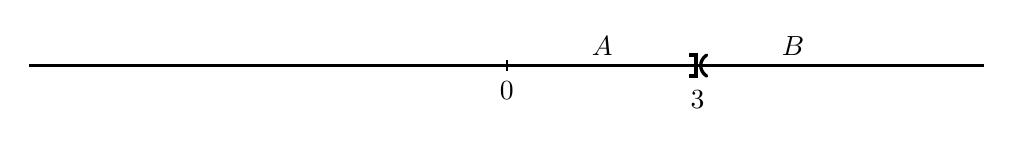
\begin{tikzpicture}
		\draw[-,thick](0,0)--(\textwidth,0);
		\foreach \x/\xtext in {0.5\textwidth /$0$}
			\draw[thick] (\x, 2pt)--(\x,-2pt) node[below]{\xtext};	
		\draw[ {-]}, very thick, black] (0,0) -- (0.7\textwidth ,0);
		\draw[ {(-}, very thick, black] (0.7\textwidth +0.5,0) -- (\textwidth,0);
		\draw (0.6\textwidth,0) node[above]{$A$};
		\draw (0.8\textwidth,0) node[above]{$B$};
		\draw (0.7\textwidth,0) node[below=2mm]{$3$};
	\end{tikzpicture}
	\\
	Dove con " ] " si intende che il numero (in questo caso 3) appartiene all'insieme di numeri $A$, mentre " ( " indica che il numero 3 non appartiene all'insieme $B$ (dalla prima regola: i due insiemi non possono condividere elementi). Visto che i due insiemi rispettano le condizioni imposte da Dedekind, la coppia $(A,B)$ forma una sezione. Il numero che divide i due insiemi \'e il numero 3, quindi la coppia di insiemi $(A,B)$ definisce il numero 3. \'E chiaro quindi che quando si usano le sezioni per definire un numero naturale, intero o razionale il numero sar\'a il valore massimo contenuto nell'insieme $A$, in quanto un qualunque numero naturale, intero o razionale \'e anche un numero razionale, quindi, per le condizioni imposte da Dedekind, sar\'a contenuto in $A$ appunto. Diverso \'e per i numeri irrazionali visto che, dalle condizioni, $A$ e $B$ non possono contenere numeri irrazionali. In quel caso il numero non sar\'a contenuto in $A$ n\'e in $B$, quindi divider\'a i due insiemi. \\
	Prima di mostrare la costruzione delle sezioni di Dedekind per il numero $\sqrt{2}$ riportiamo la dimostrazione della sua irrazionalit\'a. 
	%La dimostrazione infatti, trovata gi\'a dalla scuola pitagorica secoli fa, \'e tale da non richiedere particolari conoscenze, quindi abbastanza semplice da essere capita da chiunque:
	\begin{mdframed}[linewidth=1.5pt]
		\begin{center}		
			\textbf{\large \boldmath$\sqrt{2}$ \'e irrazionale}		
		\end{center}
		\noindent La dimostrazione \'e per assurdo, cio\'e si suppone che $\sqrt{2}$ sia razionale e si trova una contraddizione. Se $\sqrt{2}$ fosse razionale si potrebbe scrivere:
		\begin{gather*}
			\sqrt{2}=\frac{a}{b}\Rightarrow
			2=\frac{a^2}{b^2}\Rightarrow
			2b^2=a^2
		\end{gather*}
		Dimostriamo ora che questo non \'e possibile, cio\'e che \'e la contraddizione che cercavamo: considerando un generico numero $n$, nella fattorizzazione in numeri primi di $n^2$ l'esponente del 2 \'e un numero pari: se supponiamo che la fattorizzazione in numeri primi di $n$ sia
		\begin{gather*}
			n=2^{a}\times 3^{b}\times ...
		\end{gather*}	
		Allora la fattorizzazione di $n^2$ \'e:
		\begin{gather*}
			n^2=2^{2a}\times 3^{2b}\times ...
		\end{gather*}		
		L'esponente del $2$ \'e $2a$, quindi un numero pari. Un esempio:
		\begin{gather*}
			72=2^3\times 3^2\Rightarrow 72^2=2^6\times 3^4
		\end{gather*}
		Dunque nella fattorizzazione sia di $b^2$ che di $a^2$ il 2 ha esponente pari. Dunque l'equivalenza:
		\begin{gather*}
			2b^2=a^2
		\end{gather*}
		non pu\'o valere, infatti:
		\begin{gather*}
			b=2^a\times 3^b\times ...\\
			b^2=2^{2a}\times 3^{2b}\times ...\\
			2b^2=2^{2a+1}\times 3^{2b}\times ...
		\end{gather*} 
		Cio\'e nella fattorizzazione di $2b^2$ il $2$ ha esponente dispari mentre abbiamo dimostrato pocanzi che il $2$ nella fattorizzazione di $a^2$ ha esponente pari. Sapendo che due numeri uguali hanno fattorizzazione uguale, \'e una contraddizione dire $2b^2=a^2$ per via degli esponenti del $2$, pari in $a^2$ e dispari in $2b^2$; visto che hanno fattorizzazione diversa i due numeri devono essere diversi.\\
		Abbiamo dimostrato che $\sqrt{2}$ non pu\'o essere razionale, quindi deve essere irrazionale.
	\end{mdframed}
	\newpage
	\noindent Passiamo ora alla costruzione della sezione di Dedekind per il numero $\sqrt{2}$\\
	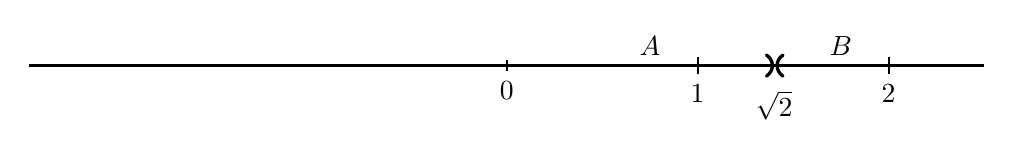
\begin{tikzpicture}
		\draw[-,thick](0,0)--(\textwidth,0);
		\foreach \x/\xtext in {0.5\textwidth /$0$}
			\draw[thick] (\x, 2pt)--(\x,-2pt) node[below]{\xtext};
		\foreach \x/\xtext in {0.9\textwidth /$2$,0.7\textwidth /$1$}
			\draw[thick] (\x, 3pt)--(\x,-3pt) node[below]{\xtext};	
		\draw[ {-)}, very thick, black] (0,0) -- (0.78\textwidth ,0);
		\draw[ {(-}, very thick, black] (0.78\textwidth +0.5,0) -- (\textwidth,0);
		\draw (0.65\textwidth,0) node[above]{$A$};
		\draw (0.85\textwidth,0) node[above]{$B$};	
		\draw (0.78\textwidth,0) node[below=2mm]{$\sqrt{2}$};
	\end{tikzpicture}
	\\
	In questo caso $\sqrt{2}$ non appartiene n\'e a $A$ n\'e a $B$, altrimenti non varrebbero le condizioni di Dedekind. Essendo il numero $\sqrt{2}$ l'unico numero che divide $A$ e $B$, la sezione $(A,B)$ definisce il numero $\sqrt{2}$.\\
	Vediamo ora come trovare l'espressione di un numero irrazionale identificato dalle sezioni $(A,B)$ prendendo in esempio $\sqrt{2}$. Concentriamoci su $A$: non contiene $\sqrt{2}$ ma contiene tutti i numeri precedenti a $\sqrt{2}$. Cio\'e \'e possibile avvicinarsi sempre pi\'u a $\sqrt{2}$ senza arrivare mai al valore preciso (cosa impossibile in quanto ha infinite cifre decimali). \'E possibile quindi trovare un'approssimazione di $\sqrt{2}$ con un numero arbitrario di cifre decimali: per trovare un'approssimazione intera del numero (senza cifre decimali) \'e sufficiente trovare il numero naturale pi\'u grande contenuto in $A$; per trovare un'approssimazione con una cifra decimale \'e sufficiente trovare il pi\'u grande numero razionale con una cifra decimale; ugualmente, per trovare un'approssimazione con due cifre decimali \'e sufficiente trovare il pi\'u grande numero razionale con due cifre decimali e cos\'i via. Nel caso di $\sqrt{2}$, $A$ contiene tutti i numeri minori di $\sqrt{2}$, da cui \'e possibile estrapolare le approssimazioni:
	\begin{gather*}
		\text{Il pi\'u grande intero: } 1\\
		\text{Il pi\'u grande razionale con un decimale: } 1.4\\
		\text{Il pi\'u grande razionale con due decimali: } 1.41\\
		\text{Il pi\'u grande razionale con tre decimali: } 1.414\\
		...
	\end{gather*}
	%(Ogni numero con una quantit\'a finita di decimali \'e rappresentabile con una frazione, quindi \'e razionale)\\
	Ovviamente considerando le approssimazioni in $A$ si arrotonda per difetto, mentre considerando quelle in $B$ per eccesso.
	\newpage
	\noindent Scostandosi per un momento dalle sezioni di Dedekind, c'\'e un'interessante dimostrazione nell'ambito dei numeri irrazionali: $0.\overline{9}=1$. Attenzione: \'e un'uguaglianza e significa proprio che i due numeri sono  uguali, non che "\textit{$0.\overline{9}$ \'e un'approssimazione di $1$}". \'E controintuitivo a prima vista, ma forniamo alcune dimostrazioni:
	\begin{mdframed}[linewidth=1.5pt]
		\begin{center}
			{\large \boldmath$0.\overline{9}=1$}
		\end{center}
		\noindent \textbf{Dimostrazione 1:}\\
		\begin{gather*}
			1=\frac{9}{9}=9\times \frac{1}{9}=9\times 0.1111...=0.9999...=0.\overline{9}
		\end{gather*}
		\\\textbf{Dimostrazione 2:}\\
		Assegniamo il valore: $c=0.999...$
		\begin{gather*}
			10c=9.999...\\
			10c-c=9.999...-0.999...\\
			9c=9\\
			c=1
		\end{gather*}
		Ma inizialmente avevamo $c=0.999...$, ora ci ritroviamo $c=1$, segue quindi $0.999...=1$\\ \\
		\textbf{Dimostrazione 3 (per assurdo):}\\
		Dimostriamo per assurdo che $0.\overline{9}=1$, partendo quindi dall'opposto:		
		\begin{gather*}
			0.\overline{9}\neq 1\\
			0.\overline{9}\times 9\neq 1\times 9\\
			0.\overline{9}\times 9+0.\overline{9}\neq 1\times 9+ 0.\overline{9}\\
			0.\overline{9}\times 9+0.\overline{9}\neq 9.\overline{9}\\
			0.\overline{9}\times (9+1)\neq 9.\overline{9}\\
			0.\overline{9}\times 10\neq 9.\overline{9}\\
			9.\overline{9}\neq 9.\overline{9}
		\end{gather*}
			Troviamo quindi un assurdo. Visto che $0.\overline{9}\neq 1$ porta ad una contraddizione, deve valere l'enunciato opposto, quindi $0.\overline{9}=1$.		
	\end{mdframed}
	Ora che abbiamo visto le sezioni di Dedekind e come definire un numero irrazionale, vediamo la dimostrazione di $0.\overline{9}=1$ con le sezioni:
	Il numero $0.\overline{9}$ \'e definito da una sezione di Dedekind, di cui il primo  insieme contiene tutti i numeri minori di $0.\overline{9}$, quindi tutti i numeri nella forma $0.\overline{9}-n$ dove con $n$ intendiamo un numero generico maggiore di $0$.\\
	Il numero $1$, ugualmente, \'e definito da una sezione di Dedekind di cui il primo insieme contiene tutti gli elementi precedenti a $1$, quindi nella forma $1-n$.
	\newpage
	\noindent Chiamando $A$ il primo insieme della sezione di Dedekind di $0.\overline{9}$ e $B$ il primo insieme della sezione di Dedekind di $1$:
	\begin{gather*}
		A=\{x\in \mathbb{Q}:x<0.\overline{9}\}=\{x\in \mathbb{Q}:x=0.\overline{9}-n \text{ con }n\in \mathbb{R}\}\\
		B=\{x\in \mathbb{Q}:x<1\}=\{x\in \mathbb{Q}:x=1-n \text{ con }n\in \mathbb{R}\}
	\end{gather*} 
	Dimostrando che $A=B$, si dimostra che la sezione di Dedekind di $1$ e di $0.\overline{9}$ \'e la stessa, quindi che $1$ e $0.\overline{9}$ sono lo stesso numero. Dimostriamo $A=B$ al solito modo: $A\subset B$ e $B\subset A$.\\
	Sicuramente vale $A\subset B$, in quanto gli elementi di $A$ sono tutti i numeri $x<0.\overline{9}$, ma tutti i numeri minori di $0.\overline{9}$ sono anche minori di $1$, quindi appartengono anche all'insieme $B$.\\
	Ogni elemento $m$ di $B$ invece \'e tale per cui $m<1$, sapendo che $m$ \'e un razionale lo posso scrivere come $m=\frac{a}{b}$ e quindi $\frac{a}{b}<1$ (dove $b>a$ altrimenti $\frac{a}{b}>1$. Consideriamo anche $b>0$, supponendo, quando si tratta di un numero negativo, di avere $a<0$ invece di $b<0$). Serve dare alcune disuguaglianze prima di procedere:
	\begin{gather*}
		1-\frac{a}{b}=\frac{b-a}{b}\geq \frac{1}{b}>\frac{1}{10^b}
	\end{gather*}
	La prima uguaglianza \'e semplicemente da definizione di somme tra frazioni. Invece $\frac{b-a}{b}\geq \frac{1}{b}$ segue dal fatto gi\'a citato che $b>a$ e da $a,b\in \mathbb{Z}$, cio\'e sono interi (stiamo lavorando con i razionali, frazioni di interi), chiaramente $b-a>1$ e quindi segue anche la disuguaglianza tra le frazioni. Invece  $\frac{1}{b}>\frac{1}{10^b}$ segue dal fatto che pi\'u aumenta il denominatore e pi\'u la frazione diventa piccola: $\frac{1}{10}=0.1$ mentre $\frac{1}{100}=0.01$. Sappiamo che $b>0$, da cui segue che $10^b>b$ (non sarebbe vero se $b$ fosse negativo), segue quindi che $\frac{1}{b}$ ha un denominatore pi\'u piccolo di $\frac{1}{10^b}$ e quindi che vale la disuguaglianza di cui sopra. Trovate queste disuguaglianze ce ne serviamo per scrivere:
	\begin{gather*}
		\text{Visto che }1-\frac{a}{b}>\frac{1}{10^b}\\
		\text{Sposto i termini:\quad } \frac{a}{b}<1-\frac{1}{10^b}
	\end{gather*} 
	Ma visto che:
	\begin{gather*}
		1-\frac{1}{10^b}=0.(9)_b<0.\overline{9}
	\end{gather*}	
	Infatti sappiamo che $\frac{1}{10^b}=0.000...1$ con $b-1$ zeri, quindi $1-\frac{1}{10^b}$ \'e uguale a $0.99999...$ dove $9$ compare $b$ volte, che \'e un valore minore di $0.\overline{9}$. Segue quindi che i numeri $\frac{a}{b}$ minori di $1$ sono anche minori di $0.\overline{9}$, quindi che gli elementi dell'insieme $B$ (minori di 1) appartengono anche all'insieme $A$ (minori di $0.\overline{9}$), cio\'e $B\subset A$.\\
	Abbiamo quindi dimostrato che $A=B$, cio\'e che $0.\overline{9}$ e $1$ hanno uguale sezione di Dedekind, segue che i due numeri sono uguali.
	\newpage
	\subsubsection{Operazioni sui reali}
	Definiamo ora le operazioni con i numeri reali. In questo caso non dobbiamo preoccuparci della buona definizione, in quanto non stiamo pi\'u lavorando con classi di equivalenza.\\
	Per definire le operazioni \'e sufficiente lavorare con il primo dei due insiemi della sezione, quello contenente tutti gli elementi a sinistra del numero che definisce, in quanto il secondo insieme \'e ricavabile dal primo.\\
	Nella sezione di Dedekind i due insiemi, per le propriet\'a che devono rispettare, sono di fatto delle semirette nella retta dei numeri:	\\
	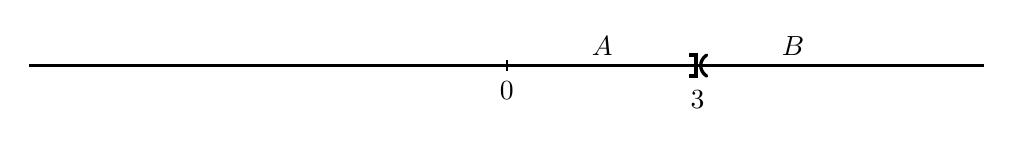
\begin{tikzpicture}
		\draw[-,thick](0,0)--(\textwidth,0);
		\foreach \x/\xtext in {0.5\textwidth /$0$}
			\draw[thick] (\x, 2pt)--(\x,-2pt) node[below]{\xtext};	
		\draw[ {-]}, very thick, black] (0,0) -- (0.7\textwidth ,0);
		\draw[ {(-}, very thick, black] (0.7\textwidth +0.5,0) -- (\textwidth,0);
		\draw (0.6\textwidth,0) node[above]{$A$};
		\draw (0.8\textwidth,0) node[above]{$B$};
		\draw (0.7\textwidth,0) node[below=2mm]{$3$};
	\end{tikzpicture}
	In questo esempio $A$ \'e una semiretta che parte da $3$ e va fino a $-\infty$, mentre $B$ \'e una semiretta che parte da $3$ (escluso) e va fino a $\infty$.\\
	Dunque la somma tra due numeri reali consiste nel traslare il primo insieme della sezione di Dedekind del primo numero in funzione del primo insieme della sezione di Dedekind del secondo numero.
	\begin{gather*}
		n=(A,B)\qquad m=(C, D)\\
		n+m=A+C=\{a+c:a\in A\wedge c\in C\}
	\end{gather*}
	La somma di due numeri \'e definita dall'insieme $\{a+c:a\in A\wedge c\in C\}$ che \'e il primo insieme della sezione di Dedekind del numero $n+m$, quindi l'insieme di tutti i numeri precedenti a $n+m$. Questo insieme \'e costituito da tutti i numeri che sono la somma di un numero in $A$, quindi il primo insieme della sezione di Dedekind di $n$, e in $C$, primo insieme della sezione di Dedekind di $m$.\\
	Per capire meglio perch\'e sia il primo insieme della sezione di Dedekind di $n+m$, \'e possibile semplificare la definizione nel caso sia $n$ che $m$ siano numeri razionali:
	\begin{gather*}
		n=(A,B)\qquad m=(C, D)\\
		n+m=A+C=\{a+m:\forall a\in A\}
	\end{gather*}	
	Cio\'e traslare l'insieme $A$ di $m$ a destra:\\
	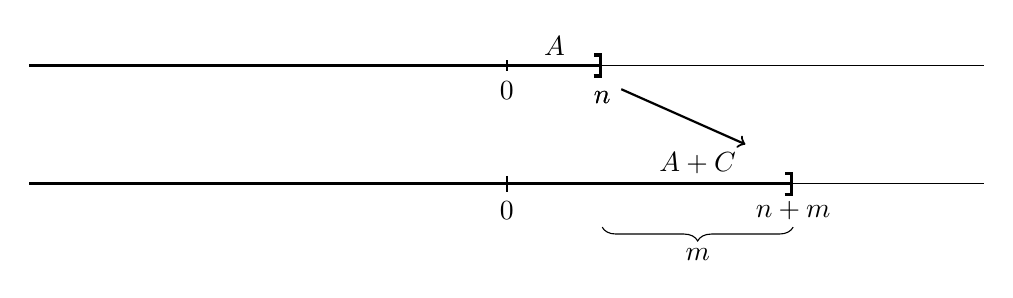
\begin{tikzpicture}
		%linea numeri		
		\draw[-,thin](0,0)--(\textwidth,0);
		%tacche
		\foreach \x/\xtext in {0.5\textwidth /$0$}
			\draw[thick] (\x, 2pt)--(\x,-2pt) node[below]{\xtext};
		%linea della A		
		\draw[ {-]}, very thick, black] (0,0) -- (0.6\textwidth ,0);
		\draw (0.55\textwidth,0) node[above]{$A$};	
		%label "n"		
		\draw (0.6\textwidth,0) node[below=2mm]{$n$};
		
		%freccia
		\draw[{->},thick](0.62\textwidth,-0.3)--(0.75\textwidth,-1);
		
		%seconda linea numeri
		\draw[-,thin](0,-1.5)--(\textwidth,-1.5);
		%tacche
		\foreach \x/\xtext in {0.5\textwidth /$0$}
			\draw[thick] (\x, -1.4)--(\x,-1.6) node[below]{\xtext};
		%linea della A		
		\draw[ {-]}, very thick, black] (0,-1.5) -- (0.8\textwidth ,-1.5);
		\draw (0.7\textwidth,-1.5) node[above]{$A+C$};	
		%label "n"
		\draw (0.6\textwidth,0) node[below=2mm]{$n$};
		%label "n+m"
		\draw (0.8\textwidth,-1.7) node[below=-1mm]{$n+m$};
		%parentesi graffa		
		\draw[decorate, decoration={brace,amplitude=5pt,raise=10pt, mirror}, yshift=0pt] (0.6\textwidth,-1.7) -- (0.8\textwidth,-1.7) node [midway, below=0.5]{$m$};
	\end{tikzpicture}
	\\
	Non \'e possibile usare questa definizione con dei numeri irrazionali, perch\'e staremmo chiedendo di spostare una semiretta di un numero con infinite cifre decimali, operazione non ben definita.
	\newpage
	\noindent L'insieme $\{a+c:a\in A\wedge c\in C\}$ mi dice infatti di prendere tutti gli elementi di $A$ e sommarli a tutti gli elementi di $C$, quindi ogni numero sempre pi\'u vicino a $n$ (appartenente a $A$) sar\'a sommato, oltre a tutti gli altri infiniti numeri, ad ogni numero sempre pi\'u vicino a $m$ (appartenente a $C$), ottenendo un insieme che contiene tutti i numeri sempre pi\'u vicini a $n+m$, cio\'e diventa l'insieme dei numeri precedenti a $n+m$, quindi il primo dei due insiemi della sua sezione di Dedekind.\\
	Per la moltiplicazione la questione \'e molto simile. Vediamo la definizione di moltiplicazione solo per due numeri reali positivi.
	\begin{gather*}
		n=(A,B)\quad m=(C,D)
	\end{gather*}	
	\begin{align*}
		 n\times m&=A\times C\\
		 		  &=\{a\times c:a\geq 0\wedge a\in A\wedge b\geq 0\wedge b\in C\}\cup \{x\in \mathbb{Q}:x<0\}
	\end{align*}
	Lavorando con numeri positivi, vengono considerati degli insiemi $A$ e $C$ solo i numeri positivi compensando la mancanza dei numeri negativi grazie all'unione con $\{x\in \mathbb{Q}:x<0\}$, cio\'e tutti i numeri razionali negativi. Nel primo insieme dell'unione abbiamo tutti i numeri sempre pi\'u vicini a $n$ e tutti i numeri sempre pi\'u vicini a $m$ (oltre che agli altri numeri positivi precedenti a $n$ e $m$) che moltiplicati tra loro sono tutti i numeri che si avvicinano sempre di pi\'u a $n\times m$, definendo quindi il primo dei due insiemi della sezione di Dedekind di $n\times m$ e quindi definendo proprio il numero $n\times m$.
	\newpage
	\subsection{Numeri complessi}
	Concludiamo la costruzione dei numeri con l'insieme dei numeri complessi:
	\begin{gather*}
	 	\mathbb{C}=\{i,1+i, -1-i, ...\}\\
	 	i=\sqrt{-1}
	 \end{gather*}
	 I numeri complessi sono nella forma $a+ib$, con $i$ che viene chiamata l' "\textit{unit\'a immaginaria}". Anche qui, similmente alle altre costruzioni, definiamo un numero complesso $n$ come una coppia di numeri reali $(a,b)$ tali che:
	 \begin{gather*}
	 	n=a+ib
	 \end{gather*}
	 Con questa notazione, $a$ viene detto \textit{parte reale}, mentre $b$, visto che \'e moltiplicata per l'\textit{unit\'a immaginaria}, viene chiamata \textit{parte immaginaria}.
	 \subsubsection{Operazioni sui complessi}
	 Quando si lavora con numeri complessi \'e possibile supporre di lavorare con polinomi di incognita $i$. Cosa significa? Significa che la somma e il prodotto tra numeri complessi segue le stesse regole della somma e del prodotto tra polinomi. Un esempio:
	 \begin{gather*}
	 	(1+x)+(3+2x)=(1+3)+(1+2)x=4+3x
	 \end{gather*}
	 Che \'e la solita somma tra polinomi, ugualmente sommo i numeri complessi:
	 \begin{gather*}
	 	(1+i)+(3+2i)=(1+3)+(1+2)i=4+3i
	 \end{gather*}
	 Come con i polinomi in cui si sommano i termini simili (termini senza $x$ del primo polinomio con i termini senza $x$ del secondo polinomio e i termini con la $x$ del primo polinomio con i termini con la $x$ del secondo) con i complessi si sommano le parti reali tra loro e le parti immaginarie tra loro. Dando la definizione rigorosa:
	 \begin{gather*}
	 	n+m= (a,b)+(c,d)=(a+c,b+d)= (a+c)+(b+d)i
	 \end{gather*}
	 Anche per il prodotto i numeri complessi seguono le regole dei polinomi:
	 \begin{gather*}
	 	(1+x)\times(3+2x)=1\times 3+1\times 2x+x\times 3+x\times 2x=3+5x+2x^2
	 \end{gather*}
	 Ugualmente per i numeri complessi:
	\begin{align*}
	 	(1+i)\times(3+2i)=1\times 3+1\times 2i+i\times 3+i\times 2i&=3+5i+2i^2\\
	 	&=3+5i+(-2)\\
	 	&=1+5i
	 \end{align*}
	 Con l'unica differenza che sappiamo quanto vale $i^2=\sqrt{-1}^2=-1$\\
	 Fornendo di nuovo una definizione formale sulle coppie di numeri reali:
	 \begin{gather*}
	 	n+m= (a,b)(c,d)=(ac-bd,bc+ad)= (ac-bd)+(bc+ad)i
	 \end{gather*}
	 Dove il segno in $-bd$ deriva appunto da $i^2=-1$
	 
	 \newpage
	 \section{Criteri di divisibilit\'a}
	Quando parliamo di criteri di divisibilit\'a stiamo parlando di algoritmi che ci semplificano la vita quando dobbiamo valutare se un numero \'e divisibile o non \'e divisibile per un altro numero. Lo scopo di questi criteri \'e rendere pi\'u veloce e pi\'u semplice questa conclusione sulla divisibilit\'a e infatti, come ricorderete, consistono in semplici operazioni da eseguire sulle cifre.\\
	Il capitolo ha come oggetto la dimostrazione di alcuni criteri e come obbiettivo quello di fornire gli strumenti necessari per trovare i criteri di divisibilit\'a per ogni numero. Questi argomenti non vengono trattati n\'e alle superiori n\'e alle medie per l'importante bagaglio di conoscenze che richiedono, conoscenze che in parte sono state spiegate negli altri capitoli. Nonostante ci\'o \'e stato necessario semplificare gli argomenti e omettere propriet\'a e dettagli nella spiegazione per renderla il pi\'u intuitiva possibile.\\
	 Questi argomenti sono la parte conclusiva del libro, nonch\'e la parte pi\'u complicata. Sono argomenti trattati a met\'a del corso di Algebra del secondo semestre del primo anno quindi, nonostante siano adeguatamente semplificati, non c\'e da spaventarsi se non tutto \'e chiaro.
	 \newpage 
	 \subsection{Anello dei resti}
	 Abbiamo visto che quando sommiamo, moltiplichiamo o facciamo altre operazioni sui numeri, lavoriamo fondamentalmente con un insieme che definisce gli elementi su cui sto eseguendo determinate operazioni, quindi i numeri, e con l'operazione stessa, definita da regole e propriet\'a (a partire da quella di \textit{buona definizione}).\\
	 Non vi sorprender\'a sapere che esistono diverse tipologie di insiemi di numeri definiti da propriet\'a caratteristiche (tipologie che si basano fondamentalmente sul tipo di numeri su cui si lavora e sul tipo di operazioni e loro propriet\'a). Ad esempio, per dimostrare i criteri di divisibilit\'a dobbiamo lavorare con insiemi chiamati "\textit{anelli}". Non entrer\'o nel dettaglio, vi basti sapere che la principale caratteristica che ci interessa \'e quella di avere l'operazione di somma e di prodotto (non basta per\'o avere le due operazioni: i numeri naturali, ad esempio, hanno sia la somma che il prodotto ma non sono un anello).\\ \\
	 Ci poniamo ora come obiettivo quello di trovare il criterio di divisibilit\'a del 3, motivo per cui bobbiamo lavorare con l'insieme:
	 \begin{gather*}
	 	A=\{0,1,2\}
	 \end{gather*}
	Ci interessa questo insieme perch\'e i suoi elementi sono tutti i possibili resti della divisione per 3, motivo per cui si chiama "\textit{anello dei resti del 3}". Pi\'u avanti sar\'a chiaro il motivo della scelta di questo insieme, concentriamoci ora sui resti della divisione per 3. \\
	Per capire perch\'e i resti della divisione per 3 possono essere solo $0, 1, 2$ forniamo degli esempi: \'e facile trovare un esempio di un numero che diviso per $3$ dia resto 0, basta considerare un numero divisibile per 3:
	\begin{center}	
		\begin{tabular}{rr|l}
			&6&3\\\cline{3-3}
			&-6&2\\\cline{2-2}
			Resto:&0&
		\end{tabular}
	\end{center}
	Ora per trovare un numero con resto $1$ \'e sufficiente, ad esempio, trovare un numero divisibile per $3$ e aggiungere $1$, ad esempio $7$:
	\begin{center}	
		\begin{tabular}{rr|l}
			&7&3\\\cline{3-3}
			&-6&2\\\cline{2-2}
			Resto:&1&
		\end{tabular}
	\end{center}
	Ugualmente, per trovare un numero con resto $2$ \'e sufficiente sommare $2$ ad un numero divisibile per $3$ oppure sommare $1$ ad un numero con resto $1$. Ad esempio, $6$ \'e divisibile per $3$, quindi $6+2=8$ ha resto $2$, ugualmente $7$ ha resto $1$, quindi $7+1=8$ ha resto $2$:
	\begin{center}	
		\begin{tabular}{rr|l}
			&8&3\\\cline{3-3}
			&-6&2\\\cline{2-2}
			Resto:&2&
		\end{tabular}
	\end{center}
	Ugualmente trovare un numero che diviso 3 dia resto 3 significa sommare 3 ad un numero divisibile per 3 ma cos\'i facendo si ottiene un altro numero divisibile per 3. Un esempio: $6+3=9$ divisibile per $3$. Quindi dopo il resto 2 si ritorna al resto 0 e si ricomincia, quindi i resti possono essere 0, 1 e 2.\\\\
	Tornando all'insieme $A$, ho omesso un dettaglio: i suoi elementi non sono semplici numeri ma sono classi di equivalenza, cio\'e:
	\begin{gather*}
		A=\{[0], [1], [2]\}
	\end{gather*} 
	Dove la relazione considera il resto della divisione per $3$. Cio\'e:
	\begin{gather*}
		n\sim 0_A\Leftrightarrow \frac{n}{3} \text{ ha resto 0}\qquad\quad
		n\sim 1_A\Leftrightarrow \frac{n}{3} \text{ ha resto 1}\\
		n\sim 2_A\Leftrightarrow \frac{n}{3} \text{ ha resto 2}
	\end{gather*}
	Dove con $0_A$ si intende lo $0$ dell'insieme $A$, diverso dallo $0$ dei numeri interi in quanto quest'ultimo non \'e una classe di equivalenza. Ugualmente per $1_A$ e $2_A$. Quindi un certo numero $n$ \'e in relazione con $0_A$ \'e equivalente a dire che la divisione $\frac{n}{3}$ ha resto 0. Ugualmente con $1_A$ \'e equivalente ad avere resto $1$ e con $2_A$ resto $2$. Quindi possiamo scrivere le classi di equivalenza:
	\begin{gather*}
		[0]=\{n: \frac{n}{3} \text{ ha resto }0\}=\{0,3,6,9,12,...\}\\
		[1]=\{n: \frac{n}{3} \text{ ha resto }1\}=\{1,4,7,10,13,...\}\\
		[2]=\{n: \frac{n}{3} \text{ ha resto }2\}=\{2,5,8,11,14,...\}
	\end{gather*}
	Un modo pi\'u semplice di scrivere le classi di equivalenza:	
	\begin{gather*}
		[0]=\{n: \frac{n}{3} \text{ ha resto }0\}=\{n:n=3t,\text{ con }t\in \mathbb{Z}\}
	\end{gather*}
	Cio\'e ogni numero divisibile per $3$ ha resto 0, quindi appartiene alla classe $[0]$, e quindi \'e nella forma $3t$, basta pensare a $3=3\cdot 1$, $6=3\cdot 2$, ...\\
	Abbiamo poi visto che se prendo un multiplo di 3 (nella forma $3t$) e aggiungo 1 ottengo resto 1, quindi \'e possibile semplificare la classe di equivalenza $[1]$:
	\begin{gather*}
		[1]=\{n: \frac{n}{3} \text{ ha resto }1\}=\{n:n=3t+1,\text{ con }t\in \mathbb{Z}\}
	\end{gather*}	 
	Similmente con la classe di equivalenza $[2]$ \'e sufficiente sommare 2 ad un multiplo di 3:
	\begin{gather*}
		[2]=\{n: \frac{n}{3} \text{ ha resto }2\}=\{n:n=3t+2,\text{ con }t\in \mathbb{Z}\}
	\end{gather*}
	\newpage	
	\subsubsection{Somma} 
	Definiti gli elementi dell'insieme $A$ su cui stiamo lavorando, rimangono da definire le operazioni di somma e prodotto, in modo che $A$ sia un anello (come ho gi\'a detto non sono sufficienti le due operazioni, ma per altri dettagli che non riporto con la somma e il prodotto $A$ diventa un anello). \'E chiaro che la somma funziona nel solito modo se consideriamo ad esempio:
	 \begin{gather*}
	 	0+0=0\qquad 0+1=1 \qquad 1+1=2
	 \end{gather*}
	 Problema di notazione: visto che stiamo lavorando con elementi di $A$ dovremmo scrivere $[0]+[0]=[0]$, cio\'e lavorare con le classi di equivalenza. Possiamo per\'o accordarci (cosa che succede spesso) e dire che togliamo le parentesi quadre ricordandoci per\'o di star lavorando sempre con classi di equivalenza in $A$! Da ora in poi quindi scriveremo gli elementi di $A$ senza le parentesi ma intenderemo comunque le classi di equivalenza.\\
	 Ma cosa possiamo dire su $2+1$? Non pu\'o essere $2+1=3$ poich\'e $3$ non \'e un elemento di $A$ (per meglio dire: $[3]$ non \'e una classe di equivalenza che appartiene a $A$). Ricordiamo per\'o che 3, in quanto divisibile per 3, cio\'e la divisione $\frac{3}{3}$ ha resto 0, appartiene alla classe di equivalenza $[0]$; quando un numero appartiene ad una classe di equivalenza possiamo scrivere: $[3]=[0]$, o come ci siamo accordati: $3=0$. Cio\'e:
	\begin{gather*}
		3\in [0]\Leftrightarrow [3]=[0]\Leftrightarrow 3=0
	\end{gather*}	 
	Generalizzando:
	\begin{gather*}
		x\in [n]\Leftrightarrow [x]=[n]\Leftrightarrow x=n
	\end{gather*}
	Seguendo questa notazione \'e possibile dire che tutti gli elementi di una classe di equivalenza sono uguali tra loro, cio\'e:
	\begin{gather*}
		[0]=\{0,3,6,9,12,...\}\\
		\Rightarrow [0]=[3]=[6]=[9]=[12]=...\Leftrightarrow 0=3=6=9=12=...
	\end{gather*}
	Cio\'e la classe di equivalenza $[0]$ raccoglie tutti gli elementi in relazione con $0$, cio\'e tutti i numeri che hanno valore $0$ nell'insieme $A$. Quindi nonostante $0,3,6,9,...$ siano numeri diversi, visto che sono elementi della stessa classe di equivalenza in $A$ hanno tutti lo stesso valore: valgono $0_A$. Vengono chiamate anche rappresentazioni dello $0$ nell'insieme $A$.\\
	Dunque abbiamo la soluzione, visto che $[0]=[3]$ o equivalentemente $0=3$:
	 \begin{gather*}
	 	2+1=0
	 \end{gather*}
	 \newpage
	 \noindent Visto che stiamo lavorando con l'insieme $A$, non posso scrivere numeri diversi dagli elementi di $A$! Fornendo altri esempi:
	 \begin{gather*}
	 	2+2=4=1 \text{ perch\'e }4\in[1]\\
	 	2+2+1=5=2\text{ perch\'e }5\in[2]\\
	 	2+2+2=6=0 \text{ perch\'e }6\in[0]
	 \end{gather*} 
	  Il nome "\textit{anello}" deriva appunto dal fatto che dopo il 2 (l'elemento massimo in $A$) si rinizia da $0$, chiudendo un virtuale anello matematico. Un altro metodo per risolvere le somme \'e fare una tabella di corrispondenze tra i numeri e gli elementi di $A$:
	 \begin{center}
	 	\begin{tabular}{c|c|c|c|c|c|c|c|c|c|c|c|c}
	 		$\mathbb{N}$&0&1&2&3&4&5&6&7&8&9&10&11\\\cline{1-13}
	 		$A$&0&1&2&0&1&2&0&1&2&0&1&2
	 	\end{tabular}
	 \end{center}
	 Tornando alla somma $2+1$ nei naturali vale $2+1=3$, cercando il corrispondente del $3$ nel nostro anello $A$ troviamo che $3=0$ e quindi $2+1=0$. Ugualmente, $2+2=4$ nei naturali, quindi in $A$ vale $2+2=1$, visto che $4=1$ dalla tabella.\\
	 Quindi per quanto riguarda la somma tra classi di equivalenza si definisce:
	\begin{gather*}
		[a]+[b]=[a+b]
	\end{gather*}
	Che \'e esattamente il modo con cui le abbiamo risolte noi senza parentesi (come da convenzione). Se le rivediamo con le parentesi:
	\begin{gather*}
		2+1=[2]+[1]=[2+1]=[3]=[0]=0
	\end{gather*}
	 Somme di questo genere non sono particolarmente complesse, pi\'u ostiche sono somme con numeri pi\'u grandi, in cui non \'e immediato capire in quale classe di equivalenza appartengono: $42+620$ ad esempio. Esiste comunque un modo per semplificare il calcolo: abbiamo visto che se un numero $x$ appartiene a una certa classe di equivalenza $[n]$, allora anche $x+3$ appartiene alla classe di equivalenza $[n]$; allo stesso modo anche $x-3$ appartiene alla stessa classe di equivalenza ($6\in [0] \Rightarrow 6-3=3\in [0]$). Allo stesso modo se sottraggo o aggiungo un multiplo di $3$ il risultato continua ad appartenere alla stessa classe di equivalenza:
	\begin{gather*}
	 	9\in [0]\\
	 	\Rightarrow 9-3=6\in [0]\\
	 	\Rightarrow 6-3=3\in [0]\\
	 	\Rightarrow 9-6=9-(3\times 2)=3\in [0]
	 \end{gather*} 
	 Prendiamo ora in esempio il numero $42$ e cerchiamo di capire in quale classe appartiene: per semplificare sensibilmente la somma \'e necessario sottrarre un multiplo di $3$:
	\begin{gather*}
	 	42\in [n]\\
	 	\Rightarrow 42-6=42-(3\times 2)=36\in [n]
	 \end{gather*} 	  
	\newpage	 
	 \noindent \'E gi\'a chiaro che, visto che 36 appartiene alla stessa classe di equivalenza di 42 e visto che 36 \'e divisibile per 3, 42 apparterr\'a alla classe $[0]$, in quanto 36 appartiene alla classe $[0]$ (appunto perch\'e \'e divisibile per 3) e quindi $[n]=[0]$. Se consideriamo ora 620:
	 \begin{gather*}
	 	620\in [n]\\
	 	\Rightarrow 620-(3\times 200)=620-600=20\in [n]\\
	 	\Rightarrow 20-(3\times 6)=20-18=2\in [n]\\
	 	\Rightarrow 2\in [2]\Rightarrow 620\in[2]
	 \end{gather*} 
	 Sottraendo diversi multipli di 3 otteniamo che $620$ \'e nella stessa classe di equivalenza di $2$, il quale ovviamente appartiene alla classe di equivalenza $[2]$, da cui segue appunto $620\in [2]$.\\
	 Visto che $42\in [0]$ e $620\in [2]$ possiamo riscrivere:
	\begin{gather*}
		42+620=0+2=2
	\end{gather*}
	 Verifichiamo che il risultato della somma $42+620=662$ abbia resto 2{\vspace{-10pt}}:\\
	 \begin{center}	
		\begin{tabular}{rr|l}
			&662&3\\ \cline{3-3}
			&-660&220\\ \cline{2-2}
			Resto:&2&
		\end{tabular}
	\end{center}
	{\large \textbf{Buona definizione}}\\
	Controlliamo ora se la somma \'e \textit{ben definita}, cio\'e se il risultato non cambia in funzione dell'elemento della classe di equivalenza con cui si lavora. Ad esempio, visto che:
	\begin{gather*}
		[1]=\{1,4,7,10,13,...\}\\
		[2]=\{2,5,8,11,14,...\}
	\end{gather*}
	Allora deve valere:
	\begin{gather*}
		2+1=5+1=5+4=...
	\end{gather*}
	Appunto perch\'e $2$ e $5$ appartengono alla stessa classe di equivalenza, cos\'i come $1$ e $4$. Dimostrare per\'o che $2+1=5+4$ non assicura che la propriet\'a di buona definizione valga con tutti gli elementi. Per dimostrarlo globalmente \'e necessario usare la definizione di classi di equivalenza:
	\begin{gather*}
		a\in [n]\Leftrightarrow a=3t+n\\
		b\in [m]\Leftrightarrow a=3t+m
	\end{gather*}
	Consideriamo quindi due elementi $a$ e $b$ in due generiche classi di equivalenza $[n]$ e $[m]$ (di quelle contenute in $A$, quindi $[0]$ o $[1]$ o $[2]$), quindi $a\in[n]$ e $b\in [m]$, da cui segue che $[a]=[n]$ e $[b]=[m]$. Per valere la propriet\'a di buona definizione deve valere:
	\begin{gather*}
		[a]+[b]=[a+b]=[m+n]=[m]+[n]
	\end{gather*}
	Appunto perch\'e $a$ e $n$ sono nella stessa classe di equivalenza e anche $b$ e $m$ sono nella stessa classe di equivalenza. \\Dunque se vale $[a+b]=[m+n]$ l'operazione di somma non dipende dall'elemento della classe di equivalenza, che \'e un rappresentante del valore della classe di equivalenza, e quindi la funzione \'e ben definita.
	\newpage
	\noindent Visto che $a\in [n]$ allora vale $a=3t+n$, e $b\in [m]$ allora $b=3s+m$ (con $a$ uso $t$ e con $b$ uso $s$ perch\'e potrebbero avere valori diversi), allora \'e possibile riscrivere:
	\begin{gather*}
		a+b=(3t+n)+(3s+m)=3(t+s)+n+m
	\end{gather*}
	\'E possibile riscrivere $t+s=v$ e ottenere:
	\begin{gather*}
		a+b=3v+(n+m)
	\end{gather*}
	Ma dalla definizione di classe di equivalenza:
	\begin{gather*}
		a+b=3v+(n+m)\Leftrightarrow (a+b)\in [n+m]
	\end{gather*}
	Inoltre $(a+b)\in [n+m]$ \'e equivalente a $[a+b]=[n+m]$ che era quello che volevamo dimostrare.\\
	\subsubsection{Prodotto}
	Per la moltiplicazione la cosa \'e analoga:
	\begin{gather*}
		1\times 1=1\qquad 2\times 1=2\qquad 0\times 0=0
	\end{gather*}
	I problemi arrivano con prodotti nella forma:
	\begin{gather*}
		2\times 2=4
	\end{gather*}
	Anche qua ricorriamo alle classi di equivalenza e, ricordando che $4\in [1]$:
	\begin{gather*}
		2\times 2=4=1
	\end{gather*}
	Analogamente alla somma, il prodotto si definisce:
	\begin{gather*}
		[a]\times[b]=[a\times b]
	\end{gather*}
	Appunto perch\'e implicitamente lo abbiamo risolto cos\'i:
	\begin{gather*}
		2\times 2=[2]\times [2]=[2\times 2]=[4]=[1]=1
	\end{gather*}	
	
	{\noindent \large \textbf{Buona definizione}}\\
	Controlliamo se il prodotto \'e \textit{ben definito}. Verifichiamo, ad esempio:
	\begin{gather*}
		[1]=\{1,4,7,10,13,...\}\\
		[2]=\{2,5,8,11,14,...\}
	\end{gather*}
	Per cui deve valere:
	\begin{gather*}
		2\times 1=5\times 1=5\times 4=...
	\end{gather*}
	Perch\'e $2$ e $5$ appartengono a $[2]$, e $1$ e $4$ appartengono a $[1]$. \\
	La dimostrazione della buona definizione ricalca quella data con la somma: consideriamo $a\in [n]$ e $b\in [m]$, quindi $[a]=[n]$ e $[b]=[m]$. Per valere la propriet\'a di buona definizione deve valere:
	\begin{gather*}
		[a]\times[b]=[a\times b]=[m\times n]=[m]\times[n]
	\end{gather*}
	Da $a\in [n]$ segue $a=3t+n$, e da $b\in [m]$ segue $b=3s+m$, dunque:
	\begin{align*}
		a\times b=(3t+n)\times(3s+m)&=3t\cdot 3s+3t\cdot m+n\cdot 3s+n\cdot m\\
									&=3(3ts+tm+sn)+nm
	\end{align*}
	Riscrivo $v=3ts+tm+sn$ e ottengo: $a\times b=3v+(n\times m)$ e dalla definizione di classe di equivalenza:
	\begin{gather*}
		a\times b=3v+(n\times m)\Leftrightarrow (a\times b)\in [n\times m]
	\end{gather*}
	Inoltre $(a \times b)\in [n\times m]$ \'e equivalente a $[a\times b]=[n\times m]$ che era quello che volevamo dimostrare.
	\newpage 
	\subsection{Dimostrazione dei criteri di divisibilit\'a}
	\subsubsection{Criterio di divisibilit\'a per 3}
	Arriviamo ora al nocciolo della questione. Abbiamo visto che i numeri in relazione con $0_A$ sono i numeri che divisi per $3$ hanno resto 0, equivalentemente sono divisibili per $3$, quindi nella forma $3t$ con $t\in \mathbb{Z}$. Quindi se  un numero \'e divisibile per $3$ deve essere in relazione con $0_A$. La cosa appare ovvia, ma come possiamo sapere, ad esempio, se il numero $167293$ \'e in relazione con $0_A$? Potremmo sottrarre multipli di 3 finch\'e non si ottiene un numero sufficientemente piccolo da capire a occhio a che classe di equivalenza appartiene, ma la questione diventa troppo complicata ricordando che il senso dei criteri di divisibilit\'a \'e proprio trovare un modo semplice di determinare la divisibilit\'a di un numero. Una soluzione al problema consiste nello scrivere il numero come somma delle sue cifre
	\begin{gather*}
		n=n_0+n_1\times 10+n_2\times 10^2+n_3\times 10^3+...
	\end{gather*} 
	Un esempio:
	\begin{align*}
		4132=&2+3\times 10+1\times 10^2+4\times 10^3\\
		=&2+30+100+4000
	\end{align*} 
	Ora la classe di equivalenza di $n$, che corrisponde al resto della divisione $\frac{n}{3}$, \'e riscrivibile come:
	\begin{gather*}
		[n]=[n_0+n_1\times 10+n_2\times 10^2+n_3\times 10^3+...]
	\end{gather*}
	Infatti visto che vale l'uguaglianza tra $n$ e la sua scomposizione, vale l'uguaglianza anche tra le rispettive classi di equivalenza, cio\'e i due numeri hanno lo stesso resto se divisi per 3. Per come sono definite le operazioni \'e possibile dividere le parentesi:
	\begin{align*}
		[n]&=[n_0+n_1\times 10+n_2\times 10^2+n_3\times 10^3+...]\\
		&=[n_0]+[n_1]\times [10]+[n_2]\times [10]^2+[n_3]\times [10]^3+...
	\end{align*}
	Stiamo lavorando con le classi resto di $3$, sappiamo che $[10]=[1]$, cio\'e $\frac{10}{3}$ ha resto 1, quindi possiamo riscrivere:	
	\begin{align*}
		[n]&=[n_0]+[n_1]\times [10]+[n_2]\times [10]^2+[n_3]\times [10]^3+...\\
		&=[n_0]+[n_1]\times [1]+[n_2]\times [1]^2+[n_3]\times [1]^3+...\\
		&=[n_0]+[n_1\times 1]+[n_2\times 1^2]+[n_3\times 1^3]+...\\
		&=[n_0]+[n_1]+[n_2]+[n_3]+...\\
		&=[n_0+n_1+n_2+n_3+...]
	\end{align*}	
	Queste semplificazioni derivano dalla definizione delle operazioni. L'ultima riga sta dicendo che $[n]$ \'e la stessa classe di equivalenza della somma delle sue cifre. Cio\'e che $\frac{n}{3}$ ha lo stesso resto di $\frac{n_0+n_1+n_2+...}{3}$ e quindi che $n$ \'e divisibile per 3 se lo \'e $n_0+n_1+n_2+...$, cio\'e se $[n_0+n_1+n_2+...]=[0]$\\
	Questa \'e la formalizzazione del solito criterio che dice che un numero $n$ \'e divisibile per 3 se la somma delle sue cifre \'e divisibile per 3. Abbiamo riproposto il criterio dicendo che la somma delle cifre di $n$ deve appartenere a $[0]$, cio\'e divisa per 3 deve avere resto 0.
	\newpage
	\subsubsection{Criterio di divisibilit\'a per 5}
	La questione \'e esattamente uguale per gli altri criteri di divisibilit\'a, la differenza \'e l'insieme su cui stiamo lavorando, che per il criterio del $5$ \'e l'insieme dei resti della divisione per 5, cio\'e:
	\begin{gather*}
		A=\{[0],[1],[2],[3],[4]\}
	\end{gather*}
	In generale i resti della divisione per un numero $n$ sono: $\{0,1,2,...,n-1\}$.\\
	Il procedimento \'e analogo: consideriamo la scomposizione del numero come somma delle sue cifre
	\begin{align*}
		[n]=[n_0]+[n_1]\times [10]+[n_2]\times [10]^2+[n_3]\times [10]^3+...
	\end{align*}	
	Visto che $10$ \'e divisibile per 5, allora vale $10\in [0]$, cio\'e la divisione $\frac{10}{5}$ ha resto 0. Quindi sostituisco $[10]=[0]$:	
	\begin{align*}
		[n]&=[n_0]+[n_1]\times [10]+[n_2]\times [10]^2+[n_3]\times [10]^3+...\\
		&=[n_0]+[n_1]\times [0]+[n_2]\times [0]^2+[n_3]\times [0]^3+...\\
		&=[n_0]
	\end{align*}
	Cio\'e $n$ appartiene alla stessa classe di equivalenza di $n_0$, la cifra delle unit\'a. Quindi $n$ \'e divisibile per 5 se $n_0$ appartiene alla classe di equivalenza  $[0]$ e quindi se \'e divisibile per 5. Visto che $n_0$ \'e una sola cifra, quindi un numero compreso tra $0$ e $9$, gli unici due valori divisibili per $5$ compresi in questo intervallo sono $0$ e $5$. Quindi si ottiene il solito criterio: $n$ \'e divisibile per 5 se lo \'e la cifra delle unit\'a, quindi se finisce con $0$ oppure $5$.
	\newpage
	\subsubsection{Criterio di divisibilit\'a per 7}
	Probabilmente non ricorderete il criterio di divisibilit\'a del 7, ma sono sicuro ricorderete che \'e difficile da ricordare.\\
	Ora \'e necessario lavorare con i resti della divisione per 7:
	\begin{gather*}
		A=\{[0],[1],[2],[3],[4],[5],[6]\}
	\end{gather*}
	Si scompone un generico numero $n$:
	\begin{align*}
		[n]=[n_0]+[n_1]\times [10]+[n_2]\times [10]^2+[n_3]\times [10]^3+...
	\end{align*}
	Questa volta \'e pi\'u semplice sfruttare la tabella invece di calcolare il resto delle divisioni passo passo:
	\begin{center}
	 	\begin{tabular}{c|c|c|c|c|c|c|c|c|c|c|c}
	 		$\mathbb{N}$&0&1&2&3&4&5&6&7&8&9&10\\\cline{1-12}
	 		$A$&0&1&2&3&4&5&6&0&1&2&3
	 	\end{tabular}
	 \end{center}
	Ricaviamo innanzitutto:
	\begin{gather*}
		[10]=[3]
	\end{gather*}
	Vogliamo semplificare il pi\'u possibile la scomposizione nella somma delle cifre, quindi ci interessa trovare i valori di $[10]$, $[10]^2$, $[10]^3$, ... per calcolare $[10]^2$ possiamo sfruttare l'uguaglianza $[10]=[3]$:
	\begin{gather*}
		[10]^2=[3]^2=[9]=[2]
	\end{gather*}
	Nuovamente per calcolare $[10]^3$ sfruttiamo le uguaglianze ottenute:
	\begin{gather*}
		[10]^3=[10]^2\times [10]=[2]\times [3]=[6]
	\end{gather*}
	Continuo:
	\begin{gather*}
		[10]^4=[10]^2\times [10]^2=[2]\times [2]=[4]\\
		[10]^5=[10]^4\times [10]=[4]\times [3]=[12]=[5]\\
		[10]^6=[10]^5\times [10]=[5]\times [3]=[15]=[1]
	\end{gather*}	
	Da qui il pattern si ripete, infatti:
	\begin{gather*}
		[10]^7=[10]^6\times [10]=[1]\times [3]=[3]\\
		[10]^8=[10]^7\times [10]=[3]\times [3]=[9]=[2]\\
		........
	\end{gather*}
	Sostituiamo:
	\begin{align*}
		[n]=&[n_0]+[n_1]\times [10]+[n_2]\times [10]^2+[n_3]\times [10]^3+...\\
		   =&[n_0]+[n_1]\times [3]+[n_2]\times [2]+[n_3]\times [6]+...\\
		   =&[n_0+n_1\times 3+n_2\times 2+n_3\times 6+n_4\times 4+n_5\times 5+\\
		   &n_6+n_7\times 3+n_8\times 2+n_9\times 6+n_{10}\times 4+n_{11}\times 5+...]\\
		   =&[n_0+3n_1+2n_2+6n_3+4n_4+5n_5+\\
		   &n_6+3n_7+2n_8+6n_9+4n_{10}+5n_{11}+...]
	\end{align*}
	\newpage
	\noindent Visto che sono nella stessa classe di equivalenza, cio\'e condividono lo stesso resto se divisi per 7, $n$ \'e divisibile per $7$ se lo \'e il numero:
	\begin{gather*}
		n_0+3n_1+2n_2+6n_3+4n_4+5n_5+\\
		n_6+3n_7+2n_8+6n_9+4n_{10}+5n_{11}+...
	\end{gather*}
	\'E possibile che vi ricordiate di un criterio vagamente diverso: $n$ \'e divisibile per 7 se lo \'e il numero
	\begin{gather*}
		n_0+3n_1+2n_2-1n_3-3n_4-2n_5+\\
		n_6+3n_7+2n_8-1n_9-3n_{10}-2n_{11}+...
	\end{gather*}	
	In realt\'a \'e lo stesso criterio, poich\'e, come abbiamo gi\'a visto, sono uguali:
	\begin{gather*}
		[n]=[n+7]=[n-7]
	\end{gather*}
	Di cui abbiamo gi\'a visto un esempio:
	\begin{gather*}
		[0]=[0+7]=[7]
	\end{gather*}
	Infatti sia $0$ che $7$ sono divisibili per $7$, quindi appartengono entrambi alla classe $[0]$, dunque \'e possibile scrivere appunto $[0]=[7]$. Ma \'e possibile scrivere anche:
	\begin{gather*}
		[0]=[0-7]=[-7]
	\end{gather*}
	Infatti anche $-7$ \'e divisibile per $7$, quindi appartiene alla classe $[0]$ e quindi $[-7]=[0]$. Dunque:
	\begin{gather*}
		[6]=[6-7]=[-1]\\
		[4]=[4-7]=[-3]\\
		[5]=[5-7]=[-2]
	\end{gather*}
	Dunque il numero che avevamo trovato
		\begin{gather*}
		n_0+3n_1+2n_2+6n_3+4n_4+5n_5+\\
		n_6+3n_7+2n_8+6n_9+4n_{10}+5n_{11}+...
	\end{gather*}
	\'e nella stessa classe di equivalenza di:
		\begin{gather*}
		n_0+3n_1+2n_2-1n_3-3n_4-2n_5+\\
		n_6+3n_7+2n_8-1n_9-3n_{10}-2n_{11}+...
	\end{gather*}	
	Quindi il numero $n$ \'e divisibile per $7$ se lo \'e quest'ultimo, esattamente come viene insegnato.\\
	Non \'e molto semplice ricordare questo criterio, ma non \'e l'unico. Esistono altri criteri, ne riporto uno tra i pi\'u semplici. Consideriamo:
	\begin{align*}
		n=n_0+n_1\times 10+n_2\times 10^2+n_3\times 10^3+...
	\end{align*}
	\'E possibile raccogliere $10$:
	\begin{align*}
		n&=n_0+n_1\times 10+n_2\times 10^2+n_3\times 10^3+...\\
		 &=n_0+10\times (n_1+n_2\times 10+n_3\times 10^2+...)
	\end{align*}
	Rinominando $b=(n_1+n_2\times 10+n_3\times 10^2+...)$ si ottiene:
	\begin{gather*}
		n=n_0+10\times b
	\end{gather*}
	\newpage
	\noindent Ragioniamo con le classi di equivalenza e moltiplichiamo la nuova espressione del numero $n$ per 5:
	\begin{gather*}
		[n_0+10\times b]\times [5]=[5]\cdot [n_0]+[5]\cdot [10\times b]=[5\cdot n_0]+[5\cdot 10]\times [b]
	\end{gather*}
	Ricordando che $[10]=[3]$, \'e possibile scrivere
	\begin{gather*}
		[5]\times [10]=[5]\times [3]=[15]=[1]
	\end{gather*}	
	Infatti $15$, se diviso per $7$, ha resto $1$. Dunque:
	\begin{gather*}
		[n_0+10\times b]\times [5]=[5\cdot n_0]+[b]
	\end{gather*}
	E riassumendo:	
	\begin{gather*}
		[n]\times [5]=[n_0+10\times b]\times [5]=[5n_0]+ [b]
	\end{gather*}
	Quindi:
	\begin{gather*}
		[n]\times [5]=[5n_0]+ [b]
	\end{gather*}
	Dunque se $n$ \'e divisibile per $7$, quindi $[n]=[0]$, allora $[n][5]=[0]$ e quindi anche $[5n_0]+[b]=0$, visto che sono uguali. Cio\'e affinch\'e $[n]$ sia divisibile per $7$ \'e sufficiente che $[5n_0]+[b]=0$, cio\'e che il numero $5n_0+b$ sia divisibile per 7.
	\newpage
	\section{Fonti e bibliografia}
	\begin{itemize}[label={}]
		\item \textbf{Insiemi}
			\subitem 			
			\begingroup			
			    \vspace{-20pt}
				\renewcommand{\section}[2]{•}				
				\begin{thebibliography}{10}			
				\bibitem{NaiveSetTheory} Paul R. Halmos, \textit{Naive Set Theory}, Martino publishing, 2011, ISBN: \texttt{978-1-61427-131-4}				
				\bibitem{wikipediaInsieme} Wikipedia: Set (mathematics), \\\texttt{https://en.wikipedia.org/wiki/Set\_(mathematics)}
				\bibitem{wikipediaUnione} Wikipedia: Union (set theory), 
				\\
				{\resizebox{0.8\hsize}{!}{\texttt{https://en.wikipedia.org/wiki/Union\_(set\_theory)}}}
				\bibitem{wikipediaIntersezione} Wikipedia: Intersection (set theory), 
				\\
				{\resizebox{0.8\hsize}{!}{\texttt{https://en.wikipedia.org/wiki/Intersection\_(set\_theory)}}}
				\bibitem{wikipediaComplemento} Wikipedia: Complement (set theory), \\{\resizebox{0.8\hsize}{!}{\texttt{https://en.wikipedia.org/wiki/Complement\_(set\_theory)}}}
				\bibitem{wikipediaInfinitaNumeriPrimi} Wikipedia: Euclid's theorem (Teorema dell'infinit\'a dei numeri primi), \\\texttt{https://en.wikipedia.org/wiki/Euclid\%27s\_theorem}
				\bibitem{proofwikiUnionDistributesOverIntersection} ProofWiki: Union distributes over Intersection, \\{\resizebox{0.87\hsize}{!}{\texttt{https://proofwiki.org/wiki/Union\_Distributes\_over\_Intersection}}}
				\bibitem{proofwikiDeMorgansLaw} ProofWiki: De Morgan's Laws (Set Theory)/Set Difference, \\{\resizebox{0.85\hsize}{!}{\texttt{https://proofwiki.org/wiki/De\_Morgan\%27s\_Laws\_(Set\_Theory)}}}
				\end{thebibliography}
			\endgroup
		\item \textbf{Costruzione dei numeri}
			\subitem 			
			\begingroup			
			    \vspace{-20pt}
				\renewcommand{\section}[2]{•}				
				\begin{thebibliography}{10}			
				\bibitem{NaiveSetTheory} Paul R. Halmos, \textit{Naive Set Theory}, Martino publishing, 2011, ISBN: \texttt{978-1-61427-131-4}				
				\bibitem{wikipediaNaturalNumber} Wikipedia: Natural Number, \\\texttt{https://en.wikipedia.org/wiki/Natural\_number}
				\bibitem{wikipediaInteger} Wikipedia: Integer, 
				\\\texttt{https://en.wikipedia.org/wiki/Integer}
				\bibitem{wikipediaRationalNumber} Wikipedia: Rational Number, \\\texttt{https://en.wikipedia.org/wiki/Rational\_number}
				\bibitem{wikipediaRealNumber} Wikipedia: Real Number, \\\texttt{https://en.wikipedia.org/wiki/Real\_number}
				\bibitem{wikipediaComplexNumber} Wikipedia: Complex Number, \\\texttt{https://en.wikipedia.org/wiki/Complex\_number}
				\bibitem{wikipediaConstructionOfRealNumber} Wikipedia: Construction of the real numbers, \\{\resizebox{0.85\hsize}{!}{\texttt{https://en.wikipedia.org/wiki/Construction\_of\_the\_real\_numbers}}}			
				\bibitem{wikipediaDedekindCut} Wikipedia: Dedekind cut, \\\texttt{https://en.wikipedia.org/wiki/Dedekind\_cut}
				\newpage 
				\bibitem{wikipediaSquareRootOf2} Wikipedia: Square root of 2, \\\texttt{https://en.wikipedia.org/wiki/Square\_root\_of\_2}
				\bibitem{wikipedia0.999} Wikipedia: 0.999..., \\\texttt{https://en.wikipedia.org/wiki/0.999...}
				\end{thebibliography}
			\endgroup
		\item \textbf{Criteri di divisibilit\'a}
		\subitem 			
			\begingroup			
			    \vspace{-20pt}
				\renewcommand{\section}[2]{•}				
				\begin{thebibliography}{10}			
				\bibitem{DispenseCaranti} Andrea Caranti, \textit{Note di Algebra - Capitolo 4: Congruenze},\\
				{\resizebox{0.9\hsize}{!}{\texttt{http://www.science.unitn.it/$\sim$caranti/Didattica/Algebra-A/static/Note/Algebra.pdf}}}				
				\bibitem{wikipediaNaturalNumber} Wikipedia: Natural Number, \\\texttt{https://en.wikipedia.org/wiki/Natural\_number}
				\end{thebibliography}
			\endgroup
	\end{itemize}
	
	\afterpage{\blankpage}%blank page successiva
	\newpage
	\afterpage{\blankpage}%blank page successiva
	\newpage
	\afterpage{\blankpage}%blank page successiva
	\newpage
	\end{document}